\documentclass[11pt]{article}
\input{glyphtounicode}
\pdfgentounicode=1

\usepackage[utf8]{inputenc}
\usepackage[T1]{fontenc}
\usepackage{lmodern}
\usepackage{amsmath,amssymb}
\usepackage[margin=1in]{geometry}
\usepackage{booktabs}
\usepackage{multirow}
\usepackage{array}
\newcolumntype{L}[1]{>{\raggedright\arraybackslash}p{#1}}
\usepackage{graphicx}
\usepackage[section]{placeins}
\usepackage[sort]{natbib}
\setlength{\bibsep}{4pt}
\bibliographystyle{apalike}
\usepackage{caption}
\captionsetup{font=small}
\usepackage[hidelinks]{hyperref}
\usepackage{setspace}
\setstretch{1.13}
\widowpenalty=10000
\clubpenalty=10000
\renewcommand{\topfraction}{0.9}
\renewcommand{\bottomfraction}{0.6}
\renewcommand{\textfraction}{0.07}
\renewcommand{\floatpagefraction}{0.8}
\newcommand{\pinc}{\overline{\mathrm{ParentInc}}}

\title{Before the Labor Market or Inside It?\\
Family Background, Earnings Dynamics, and the Return to College}
% The one place to set the address of the public repository (online appendix and replication files).
\newcommand{\repourl}{https://github.com/JiachenJin1001/family-background-earnings-china}
\author{Jiachen Jin\thanks{New York University, \texttt{jj4608@stern.nyu.edu}.
The Online Appendix (supplementary results, proofs of the formal results, and a replication guide) and the replication files are available at \href{\repourl}{\nolinkurl{github.com/JiachenJin1001/family-background-earnings-china}}.
All errors are mine.}}
\date{October 2026}

\hypersetup{pdftitle={Before the Labor Market or Inside It? Family Background, Earnings Dynamics, and the Return to College}, pdfauthor={Jiachen Jin}}
\begin{document}
\maketitle

\begin{abstract}
\noindent Among Chinese adults whom the China Family Panel Studies
links to their parents, the children of officials, managers, and
professionals (advantaged children) earn 22 percent more than other
children (less advantaged children). I ask whether this advantage is
built inside the labor market, through smaller earnings shocks or
faster earnings growth, or is in place before work begins, through access to college and the occupations a degree opens. It is in place before work begins.
Minimum-distance estimates of the earnings process of each group,
Arellano--Bond dynamic panel regressions, and fixed-effects growth
regressions show no detectable difference in the variance or the growth
of earnings. The same estimates imply that one wave of income recovers a quarter to two fifths of the coefficient
on permanent income. With parental income held fixed, correlated
random-effects regressions and entropy balancing put the premium of
advantaged children at 7 to 17 percent. To value the gap in college
completion behind it, I use the 1999 expansion of university admissions
and an instrument that interacts the growth of university seats in the
province with each birth cohort's exposure. Completion rose in both groups, from 17 to 50 percent among advantaged children and from 5 to 24 percent among less advantaged children, and added seats raised it by a similar number of percentage points in each. For a child who completed college because seats were added, college raised earnings by 0.68 log points, or 0.17 per year of college; by family background the return is 0.62 for less advantaged children and 1.14 for advantaged children. At the entropy-balanced premium of
7 percent, the gap in college completion, valued at the return to
college, accounts for between three quarters and all of the premium.\\[4pt]
\textbf{JEL:} J62, J31, I23, I24, C23. \quad \textbf{Keywords:}
intergenerational mobility; earnings dynamics;
attenuation bias; higher
education expansion; shift-share instrument; China.
\end{abstract}

\newpage

\section{Introduction}
\label{sec:intro}

In a national panel of Chinese households, children of officials, managers, and professionals earn 22 percent more than other children. There are two places to look for the source. One is the labor market itself: these children might face smaller earnings
shocks, recover from bad years faster, or climb steeper career paths.
The other is the years before work, if what their families
secure is schooling, and above all a seat at university, which
admission quotas kept scarce until 1999. The difference matters. Protection inside the labor
market would operate throughout a career, and no single reform at the
start of adult life could undo it. An advantage settled at the
university gate depends on the rules that allocate seats. I ask which of the two the data support, and the answer is the second. I find no detectable difference between the two groups in earnings risk or in earnings growth. By earnings risk I mean the size of the shocks that
move a person's earnings around their expected path; earnings dynamics
covers risk and growth together. Most of the advantage that parental income leaves unexplained is tied to college, completed before work begins.

Throughout, advantaged children
are those with at least one parent in an official, managerial, or
professional occupation when the child was fourteen, and less advantaged children are all others. The label is about what the parents did, not what they earned: the earnings comparisons of Sections~\ref{sec:premium} to \ref{sec:mediation} hold parental income fixed, so an advantaged family here need not be a high-income family. Occupation marks family
position here for a reason specific to the parents' generation. These
parents built their careers in the 1980s and 1990s, when state pay
scales compressed wages and a family's income said little about its
standing. A parent's occupation determined the work unit, and with it housing, urban registration, and the connections that a post in government, management, or the professions carried; these are what a parent could bring to bear for a child \citep{BianLogan1996,
WuTreiman2007}.

The data are the China Family Panel Studies (CFPS), 2014 to 2022, in which 4,536 adult children are linked to their parents. I first estimate the earnings process of the two groups, by minimum
distance on the autocovariances of residual earnings and by Arellano--Bond
dynamic panel regressions. I then measure the difference in the level of earnings with parental
income held fixed, by correlated random effects and by entropy
balancing. Finally I use the 1999 expansion, in which university admissions rose
by more than 40 percent in a single year and kept growing for a decade, to learn, for each group, which children it moved into college and what college did for them. The instrument is the growth of university seats in the province interacted with the exposure of each birth cohort.
Table~\ref{tab:roadmap}
pairs each finding with the method behind it.

\begin{table}[t]
\centering
\small
\caption{The questions the paper asks and what it finds.}
\label{tab:roadmap}
\begin{tabular}{@{}L{3.2cm}L{5.8cm}L{5.0cm}c@{}}
\toprule
Question & Finding & Method & Section \\
\midrule
Earnings risk or growth by family background? & No detectable
difference in variances, autocovariances, or growth & Minimum distance
on autocovariances; Arellano--Bond GMM; nonlinear persistence;
fixed-effects growth regressions & \ref{sec:process} \\
\addlinespace
Attenuation from one wave of income? & One wave recovers a quarter
(children's process) to two fifths (parents' process) of the
coefficient on permanent income & Attenuation schedule from the
estimated process; check on a published study &
\ref{sec:measurement} \\
\addlinespace
Size of the level premium? & 7 to 17 percent with parental income held
fixed; party membership and state-sector employment add little once
parental occupation enters & Correlated random effects; entropy balancing;
competing markers; fifteen specifications & \ref{sec:premium} \\
\addlinespace
Whom did added seats admit, and what did college return? & Completion
rose in both groups (advantaged 17 to 50 percent, less advantaged 5 to 24); return 0.68 log
points (19 percent per year of college), 1.14 for advantaged and 0.62 for less advantaged children; more years in official, managerial, or professional occupations & Shift-share instrument (provincial seat
growth times cohort exposure); precision weights from the
earnings process; Anderson--Rubin sets; randomization inference; placebo instrument &
\ref{sec:expansion} \\
\addlinespace
How much of the premium is college? & All at the instrumented returns;
three quarters at the least squares return & Accounting identity over
a range of returns & \ref{sec:mediation} \\
\bottomrule
\end{tabular}
\end{table}

Among the children observed in at least three waves, 420 are advantaged and 2,103 less advantaged, and their residual earnings are equally dispersed. The fitted variances are 0.44 and 0.46, and none of the fifteen
variances and autocovariances that the five waves provide separates the groups (joint test $p = 0.32$). The earnings gap between them grows by 0.02 log points per two-year wave (SE 0.014), which is not distinguishable from zero. The estimated
process has the form documented in American panels, and about a quarter of the variance of residual
earnings reflects lasting differences between people. That share also measures how badly a single wave of income stands in for permanent income, the errors-in-variables problem that \citet{Solon1992}
documented for the United States: a regression on one wave recovers about a quarter of the
coefficient on permanent income under the earnings process estimated for the children, and a little over two fifths under the one estimated for their parents (Section~\ref{sec:measurement}). Attenuation matters here because every comparison below holds parental income fixed.

The gap in mean log annual earnings between advantaged and less advantaged
children is 0.195 log points (22 percent). Holding parental income and demographics fixed removes a fifth to three fifths of it; what remains, 0.07 to 0.15 log points or an earnings difference of 7 to 17 percent, is a premium that the family's measured income does not account for. Party membership and state-sector employment, two markers of position that
studies of Chinese stratification emphasize \citep{LiEtAl2007,
WalderLiTreiman2000}, are far more common among parents in these occupations than among other parents. On its own, each has a coefficient a little over half that of parental occupation and is not distinguishable from zero. Once parental occupation enters, neither marker changes the occupation coefficient.

The premium does not say through which channel parental occupation reaches a child's earnings, and Sections~\ref{sec:expansion} and \ref{sec:mediation} take up that question. Whether the child completes college is the main candidate. Advantaged children complete college at more than twice the rate of less advantaged children, and once the child's own college completion is added to a regression that holds parental income fixed (Section~\ref{sec:mediation}), the coefficient on parental occupation falls from 0.08 to 0.02. The regression hands more than two thirds of the premium to college completion. I do not take that at face value. College completion is
itself an outcome of family background, and children who complete college differ from those who do not in ability, preparation, and family resources that raise earnings on their own. The coefficient on college mixes the effect of a degree with these confounders and says nothing about a child who would not otherwise have
attended. So I need a change in access to college that no family chose. The 1999
expansion is one, and I ask which children it moved into
college and what college did for them.

The gap in college completion between the two groups can arise in two ways, and the design of the admission system makes the distinction
sharp. Admission was by examination score alone: the seats allotted to
a province were filled in rank order of the score, and in principle
no seat was reserved for any family. Yet before the reform 17.3 percent of advantaged children and 4.6 percent of less advantaged children completed college. One reading is that the score ranked ability. The other is that
the score ranked preparation under unequal conditions. In the China of
the 1980s and 1990s, advantaged families could offer their children
city schools, key-point high schools, and the material security to devote themselves to preparing for the examination; when seats were few and the
cutoff high, their children filled the top of the ranking, and less advantaged children clustered below the cutoff. Under either reading,
added seats lower the cutoff and admit children from below the old
one, where less advantaged children are the larger share, so their
weight among graduates rises whatever the score measures. Less advantaged children, 83 percent of all children, were 57 percent of the graduates in the cohorts before the reform and 75 percent of the additional graduates in the cohorts after it. The ratio of the completion rate of advantaged children to that of less advantaged children fell from 3.7 in the cohorts born before 1981, who reached college age before the reform, to 2.1 in those born in 1981 or later.

The two readings differ
in what the newly admitted children gain. If the score ranked ability,
the children admitted at the margin gain less from college than those
admitted before them. If it ranked preparation, the newly admitted children, once in college and given the
conditions that advantaged children already had, can hold the same jobs and earn a return no lower
than the average. Both can be true at once. What
separates them is the return to college for the children the
added seats admitted, and the 1999 expansion, which added seats at
different rates across provinces, supplies it. With that return comes an answer to the question asked of any expansion of higher education: whether it
passes the advantages of one generation to the next or opens a door
that family background had kept shut.

I organize the evidence with one
accounting identity. The premium equals the gap in college completion
between the two groups, multiplied by the return to college, plus
whatever else the parents' occupation brings, such as information,
connections, or a better institution for the same degree:
\begin{equation}
\tau \;=\; \beta^{H} \cdot \Delta M \;+\; \mathrm{Direct}.
\label{eq:hp-intro}
\end{equation}
Here $\tau$ is the premium, $\Delta M$ the gap in college
completion between advantaged and less advantaged children with the same parental income ($M$ is the
indicator for college completion, sixteen or more years of schooling), $\beta^{H}$ the return to college
for advantaged children, and Direct the direct effect: the part of the premium that reaches earnings without passing through the completion of college, including any higher value that the same degree carries for an advantaged child.

In the cohorts born in 1981 or later, 50 percent of advantaged children and 24 percent of less advantaged children completed college. Part of the rise from the pre-reform rates is a national trend, and to separate the
reform from it I use a shift-share instrument: a
provincial measure of how much university seats grew (provincial intensity), multiplied by
the
ratio of national admissions in the year a birth cohort reached college age
to the pre-reform trend. With province and birth-year fixed effects,
the comparison is a difference-in-differences: between provinces that added more and fewer seats, across cohorts more and less exposed. In provinces that expanded more, children of both groups completed college more often. Relative to the cohorts born before 1981, an interquartile difference in provincial intensity raises the completion of the cohorts born in 1989 or later, who faced admissions about four times the pre-reform trend, by 8 percentage points among less advantaged children and by 7 among advantaged children. The instrumented return to college is 0.68 log points, or 0.17 per year of college (19 percent per year), with an Anderson--Rubin confidence set that excludes returns below 0.50; the least squares
return is 0.45. The outcome is each child's long-run level of earnings, an average over several survey waves, and an average of few waves is noisy. The earnings process estimated in the first part of the paper says how noisy. When I weight each average by the precision it implies, the return is 0.63.

The instrument identifies a local average treatment effect in the sense of \citet{ImbensAngrist1994}: a weighted average of the returns to college for compliers, the children the added seats admitted. By family background, it is 0.62 for less advantaged children and 1.14 for advantaged children (17 and 33 percent per year of college), both above the least squares return of 0.45.

The identity needs the premium and the completion gap measured on the same comparison. With less advantaged children reweighted to the parental income and demographics of advantaged children, the premium is 0.072 log points (7 percent) and the gap in college completion is 12.2 percentage points. Valued at the instrumented return for all children, 0.68, the completion gap accounts for all of the premium; valued at the least squares return, a lower benchmark, it accounts for three quarters.

A natural reading of the premium is that parents who are officials, managers, or professionals pass on their ability, and that inherited ability accounts for much of the advantage that family income leaves unexplained. The reading comes in two versions, and the evidence bears on each. In the first, ability is rewarded in the labor market directly, with or without a degree. If advantaged children are on average the more able at each level of schooling, an advantaged child should then earn more than a less advantaged child with the same schooling. The point estimates show no such gap. With parental income held fixed, advantaged and less advantaged children without a degree earn the same (a difference of 0.001 log points), and so, nearly, do advantaged and less advantaged graduates (0.024). In the second, ability decides who wins a seat, as in the first reading of the completion gap above. The children admitted only because seats were added, who had scored below the earlier cutoff, would then gain less from college than the graduates before them. I find no sign of that: their return is no lower than the least squares return. Most of the premium therefore comes through access to college, not through ability rewarded outside it; and on whether access itself reflects ability or preparation, the returns of the newly admitted favor preparation.

The expansion design rests on two assumptions: parallel trends (provinces that added more seats were not already on different trends) and exclusion (the instrument affects the
outcomes only through college). Four checks address them. A predetermined provincial measure, the census share of each province's adults who had
completed senior secondary school before the reform, reproduces the earnings results. A placebo built from pre-reform growth in examination
registrations, which I assemble from statistical yearbooks, does not predict
college completion (first-stage $F = 0.5$, compared with 18.0 for the instrument). Children with nine or fewer years
of schooling, who were never candidates for college, did not move into official, managerial, or professional occupations where seats grew faster. Controls for the export boom that followed
WTO accession leave the results unchanged.

The minimum-distance and Arellano--Bond estimates of the residual earnings
process apply to the CFPS panel the covariance-structure methods of \citet{LillardWillis1978}, \citet{MaCurdy1982},
\citet{HallMishkin1982}, \citet{AbowdCard1989}, and
\citet{MeghirPistaferri2004}, and their extension to nonlinear persistence by
\citet{ArellanoBlundellBonhomme2017}. The process looks the same in the two groups, which leaves earnings risk without a measurable role as a channel
of transmission. For the measurement
literature that begins with \citet{Solon1992} and
\citet{Zimmerman1992}, and that \citet{Mazumder2005} and
\citet{HaiderSolon2006} extended, I supply attenuation factors
estimated on Chinese earnings, which the debate over Chinese
persistence estimates \citep{GongLeighMeng2012, DengGustafssonLi2013, FanYiZhang2021,
YuanLin2013} has lacked. The work on China's college expansion has concentrated on the labor market for graduates, firms, and general-equilibrium effects \citep{CheZhang2018, KnightDengLi2017, Ma2024IER}, and on college entry, where family background is found to have kept its hold \citep{Yeung2013}, as the maximally maintained inequality hypothesis of \citet{RafteryHout1993} predicts. I ask instead which children the reform moved into college and what it returned to each group. The instrumented return per year of college is close to the instrumented returns to schooling found for China \citep{HuangTaniWeiZhu2022, FangEtAl2012}. \citet{ChenZhuWang2026} and \citet{HuangTaniWeiZhu2022} find, by matching and by an instrument built from childhood urban household registration (\emph{hukou}), that the return to college for students from less advantaged backgrounds whom the expansion admitted is at least as high as for other students. Neither design uses the variation in seat growth across provinces, and neither links the
return to a decomposition of the premium.

\section{Data}
\label{sec:data}

\subsection{Panel and income concept}
\label{sec:income}

The China Family Panel Studies (CFPS) is a biennial household panel administered by the Institute of
Social Science Survey at Peking University since 2010 \citep{XieHu2014}. Its baseline sample covers 25 provinces and, with the survey's
sampling weights, represents about 95 percent of the national
population. Respondents who move are followed under a stable person identifier, and some now live outside the baseline provinces; the sample of Section~\ref{sec:sample} spans 29 provinces. The sample conditions on panel participation (several income waves and a retrospective response), so the sampling weights no longer reproduce the population. I do not use them, and the estimates describe the sample.

The survey's measure of personal labor income changed definition in 2014.
Before 2014 the headline income variable bundles labor earnings with
transfers and asset income; from 2014 onward it covers labor income only. The
variance of log income is lower under the new concept: among all respondents aged 22 to 55 with positive income it is 1.37 in the 2012 wave and between 0.85 and 1.04 in each of the five waves from 2014. An estimator that pooled waves from before and after 2014 would attribute the change in definition to earnings
shocks. The main analysis
therefore uses the five waves from 2014 to 2022. Where a longer panel
helps (the growth-rate tests and the seven-wave persistence check), I reconstruct a measure for 2010 and 2012 that covers labor income
only, by summing the wage, bonus, self-employment, and family-business
components and leaving out transfers and asset income, and label every
estimate that uses it as coming from the
reconstructed panel; no main estimate rests on it.

\subsection{Sample and family background}
\label{sec:sample}

A child is a CFPS respondent whose father or mother can be located through the family-relationship roster and appears in a survey file in at least one wave. The grouping variable, denoted $H_i$, equals one if either parent held
an occupation in the top two major groups of China's Standard
Classification of Occupations (CSCO): heads of state organs, party
organizations, enterprises, and public institutions, or professionals and technical personnel (the counterparts of
major groups 1 and 2 of the international classification, ISCO, so the
grouping is the one that international studies of class use). Parental occupation is measured when the child was fourteen, from
retrospective questions asked in the 2012, 2020, and 2022 waves, under
the either-parent dominance convention of
\citet{EriksonGoldthorpe1992}.\footnote{For
319 children in the sample only one parent's occupation is reported; the indicator
codes them by the reported parent, which treats a missing second
parent as not advantaged and, if anything, attenuates the group
contrast.} I call children with $H_i = 1$
advantaged children and all others less advantaged children. Children
without a valid retrospective response are excluded rather than
imputed, and the sample conditions on participation in one of those
three waves.

The paper uses one sample. A child enters it with a retrospective
report, the family income of the parental household, a province for
which Section~\ref{sec:expansion} has a measure of the expansion, and
positive labor income in at least two waves between 2014 and 2022 at
ages 22 to 55. Twenty-two is the age at which a four-year graduate
enters the labor market; 55 is the middle of the three statutory
retirement ages in force over the period (50 for women in worker posts,
55 for women in cadre posts, and 60 for men). Wave by wave I trim the income distribution: log incomes below
$\log 1000$ yuan are dropped, as is the top 1 percent of log income.
The sample has 4,536 children (755 advantaged, 16.6 percent) and 12,675
child-waves, born 1961 to 1997.

Sections~\ref{sec:process} and
\ref{sec:measurement} ask about the path of earnings: its shocks, their
persistence, and its growth. Dynamic panel estimation takes at least three waves, and 2,523 children (420 advantaged) have them, with 8,649
child-waves. Sections~\ref{sec:premium} to \ref{sec:mediation} ask
about the level of earnings, which I measure at ages 30 and over. A
child's \emph{level of earnings} is the mean, over the waves at ages 30
and over, of log labor income net of survey-year effects, computed for
the children with at least two such waves; 2,774 children (453
advantaged) have one, and 1,804 children have both three waves and a
level. Section~\ref{sec:expansion} keeps all 4,536 children; those without a level of earnings help estimate its province and birth-year effects and the coefficients on its controls (Section~\ref{sec:design}).

The definition of the level of earnings makes two choices. The first is age 30.
Earnings in the twenties are a poor measure of where a career settles
\citep{HaiderSolon2006}, and they are poorest for the comparison made
here, because graduates enter the labor market later than other
children. At ages 22 to 25 many graduates are still in school or newly
hired. Postgraduate study is open only to four-year graduates: those
who go on to a master's degree start work at about 25, and those who
take a doctorate close to 30, so at ages 26 to 29 they are in their
first years of work while children of the same age without a degree
have worked for about a decade. On
the child-waves in the sample, with survey-year and age effects, the
least squares return to college is $-0.02$ log points at ages 22 to 25 (SE 0.05),
0.37 at 26 to 29, 0.46 at 30 to 34, and 0.41 at 35 to 55; it is still rising through the late twenties. The second is
the removal of survey-year effects before averaging. Mean log income at
ages 30 and over rose from 10.19 in the 2014 wave to 10.81 in the 2022
wave (by more than four fifths in nominal terms). An average of raw log income would depend on the years in which a
child happens to be observed. So I remove from each log income
the effect of its survey year, estimated on all child-waves in the
sample and centered on the overall mean so that the result stays in
log yuan, before averaging over a child's waves.

Of all advantaged children with a retrospective report and parental family income who are observed at least once
at ages 22 to 55 in a 2014--2022 wave, 45 percent satisfy every
screen and enter the sample; among less advantaged children the
figure is 42 percent. For the children with three waves the figures are
25 and 23 percent. The screens remove the two groups at nearly the
same rate, so differential selection into the sample is unlikely to drive the group
comparison. Employment does differ between the groups. Before any
earnings screen is applied, earnings are positive in 56 percent of the
person-waves of advantaged children and in 50 percent of the
person-waves of less advantaged children, and the comparison of earnings risk
is conditional on having earnings.

CFPS also records the occupations that parents hold from 2010 to 2022, which yields an alternative indicator based on the
parents' current occupations. The
two measures agree for 86 percent of the children in the sample for whom both exist, and
the disagreement is asymmetric in the direction retirement predicts:
10.2 percent of children have parents who held such an occupation when
the child was fourteen but had moved down by the observation window,
against 4.0 percent who moved up. An indicator measured after parents
have retired or moved down misclassifies some advantaged families,
which attenuates the estimated group contrast. The retrospective
indicator is therefore the baseline and the indicator based on current
occupations is used
in robustness checks; the disagreement rate also enters the
misclassification analysis of Section~\ref{sec:premrobust}.

Table~\ref{tab:desc} compares the two groups, among all children in the sample and among the children with a level of earnings. In both, advantaged children earn
about 0.2 log points more on average; they have parents with more
family income (by more than 0.4 log points), acquire more than two additional years of schooling, and complete
college at more than twice the rate of less advantaged children.
They are more urban and more often female. Birth years and the number of waves
are balanced across the groups.

\begin{table}[t]
\centering
\small
\caption{The sample: means by family background.}
\label{tab:desc}
\setlength{\tabcolsep}{5pt}
\begin{tabular}{@{}lcccc@{}}
\toprule
& \multicolumn{2}{c}{All children, ages 22 to 55} & \multicolumn{2}{c}{Children with earnings at 30 and over} \\
\cmidrule(lr){2-3}\cmidrule(lr){4-5}
& Advantaged & Less advantaged & Advantaged & Less advantaged \\
\midrule
Mean log labor income & 10.66 (0.65) & 10.45 (0.65) & 10.67 (0.64) & 10.48 (0.64) \\
$\pinc$ (log family income) & 10.99 (0.77) & 10.56 (0.74) & 11.06 (0.75) & 10.58 (0.79) \\
Years of schooling & 13.77 (3.08) & 11.56 (3.64) & 13.20 (3.32) & 10.74 (3.70) \\
College (16$+$ years) & 0.41 (0.49) & 0.18 (0.39) & 0.34 (0.47) & 0.14 (0.35) \\
Female & 0.36 (0.48) & 0.27 (0.45) & 0.30 (0.46) & 0.20 (0.40) \\
Urban (first wave) & 0.76 (0.43) & 0.55 (0.50) & 0.77 (0.42) & 0.56 (0.50) \\
Age over the waves & 34.2 (8.6) & 34.1 (8.2) & 39.7 (7.0) & 39.2 (6.6) \\
Birth year & 1984.4 (9.0) & 1984.4 (8.5) & 1979.1 (7.7) & 1979.6 (7.2) \\
Waves with labor income & 2.81 (0.84) & 2.79 (0.83) & 2.75 (0.82) & 2.70 (0.80) \\
\addlinespace
Children & 755 & 3,781 & 453 & 2,321 \\
\bottomrule
\end{tabular}

\par\smallskip
\begin{minipage}{0.92\textwidth}
\footnotesize\emph{Notes:} Standard deviations in parentheses. CFPS
2014--2022. All children: the 4,536 children with at least two waves of
positive labor income at ages 22 to 55; their labor income is the mean
of log nominal annual income in yuan over all their waves. Children
with earnings at 30 and over: the 2,774 with at least two
waves at those ages; their labor income is the level of earnings
defined in the text (net of survey-year effects, centered on the overall mean), and age and the number of waves refer to the waves
at 30 and over. Advantaged: either parent held a CSCO major group 1 or
2 occupation when the child was fourteen.
\end{minipage}
\end{table}

\subsection{Parental income and co-residence}
\label{sec:parentinc}

Parental economic resources are measured as $\pinc_i$, the mean of log
family income across all waves in which the parental household appears
in the family-economy module. I prefer family income to the parents'
personal labor income. Many parents are past working
age during the observation window, and their personal labor income is observed
in fewer waves and for fewer parents. Family income also includes the
asset and business income that a personal-earnings measure leaves out,
which matters most for advantaged families.

The family income measure has one known defect. When an adult child appears
on the same household roster as a linked parent (nearly two thirds of the child-waves in the sample), the family income figure mechanically
includes the child's own earnings, so a regression of child earnings on
$\pinc_i$ partly regresses the child on herself. I therefore construct
a second measure from the linked parents' own labor-income records,
which cannot contain the child's earnings by construction, and report
both versions. If co-residence contaminates the family measure, replacing
it with the parents' own labor income should lower the income
coefficient and raise the occupation coefficient, and it does both (Section~\ref{sec:cre}).

\section{The earnings process and family background}
\label{sec:process}

Parents in official, managerial, or professional occupations might protect their children's earnings in three ways: smaller shocks, faster recovery from a bad year, or steeper
earnings growth. This section estimates each feature separately by
family background.

\subsection{Framework}
\label{sec:framework}

Let $y_{it}$ denote log labor earnings of child $i$ in wave $t$. After
removing observables, I treat residual earnings as generated by
\begin{equation}
\tilde y_{it} \;=\; \eta_i \;+\; g_i t \;+\; v_{it} \;+\; m_{it},
\qquad v_{it} = \rho_v\,v_{i,t-1} + \varepsilon_{it},
\label{eq:unified}
\end{equation}
where $\eta_i$ is a permanent individual component, $g_i$ an
individual growth slope, $v_{it}$ a persistent AR(1) component, and
$m_{it}$ serially uncorrelated noise. Equation~\eqref{eq:unified} nests
the classical permanent--transitory model \citep{HallMishkin1982,
MaCurdy1982}, the heterogeneous-profiles specification of
\citet{Guvenen2009}, and the linear special case of the latent-state
model of \citet{ArellanoBlundellBonhomme2017}. I do not estimate
equation~\eqref{eq:unified} as a whole. Each estimator below recovers
some of its moments under its own restrictions, and I compare what they
give. The share of residual variance that is permanent governs
attenuation bias in regressions of child outcomes on parental income. The persistence of shocks
governs how fast averaging removes the transitory part. The
distribution of growth slopes $g_i$, and especially its dependence
on family background, would capture any dynamic advantage that levels
cannot.

All dynamic estimation uses residual log earnings $\tilde y_{it}$, the
residual from a pooled regression of log labor income on year fixed
effects, a quartic in age, gender and its interactions with the age
quartic, urban status, and province fixed effects, winsorized at the
first and ninety-ninth percentiles within each wave. Year effects are
common rather than group-specific, so between-group differences survive
into $\tilde y$, and the growth regression of Section~\ref{sec:abb} uses
them; the second-moment estimation additionally demeans within group and year so
that group means do not mechanically enter the autocovariances. The
level regressions of Section~\ref{sec:premium} do not use these
residuals; they include the controls directly.

\subsection{Two persistence parameters}
\label{sec:twopers}

Both dynamic estimators below target the persistence of the
\emph{transitory component}, an object easily conflated with the
persistence of observed earnings. The minimum-distance model of
Section~\ref{sec:md} fits it after attributing part of the
autocovariance to a permanent effect; the dynamic panel regression of
Section~\ref{sec:abgmm} reaches the same parameter from the other
direction, differencing the permanent component away rather than
modeling it. The AR(1) coefficient of \emph{observed residual
earnings}, which a regression without individual effects would deliver,
mixes the two components. With a permanent share
$s = \sigma^2_\eta / (\sigma^2_\eta + \sigma^2_v)$, where
$\sigma^2_\eta$ is the variance of the permanent component and
$\sigma^2_v = \sigma^2_\varepsilon/(1-\rho_v^2)$ the variance of the
transitory component in equation~\eqref{eq:feAR} below, and transitory
persistence $\rho_v$,
that coefficient is, under stationarity,
\begin{equation}
\rho_{\mathrm{obs}} \;=\; \rho_v + (1 - \rho_v)\, s,
\label{eq:rhoobs}
\end{equation}
so the observed-earnings coefficient always exceeds the transitory one
when a permanent component exists. Two estimates can be compared
only if they measure the same parameter. The minimum-distance and
Arellano--Bond estimators both measure the persistence of the
transitory component, so if they disagree, the disagreement is real.

\subsection{Permanent and transitory components}
\label{sec:md}

The baseline specification restricts \eqref{eq:unified} to a permanent
effect plus an AR(1) transitory part,
\begin{equation}
\tilde y_{it} = \eta_i + v_{it}, \qquad
v_{it} = \rho_v\, v_{i,t-1} + \varepsilon_{it}.
\label{eq:feAR}
\end{equation}
I fit $(\sigma^2_\eta, \sigma^2_\varepsilon, \rho_v)$ by minimum
distance to the vector of empirical pairwise autocovariances, which
under \eqref{eq:feAR} take the form
\begin{equation}
\mathrm{Cov}\left(\tilde y_{it}, \tilde y_{i,t+k}\right)
\;=\; \sigma^2_\eta \;+\; \rho_v^{\,k}\,
\frac{\sigma^2_\varepsilon}{1-\rho_v^2},
\qquad k = 0, 1, 2, \dots,
\label{eq:moments}
\end{equation}
so the long-lag asymptote of the autocovariance function identifies
the permanent variance and the geometric decay toward it identifies
the transitory pair. Each moment is weighted by the number of pairs of
observations behind it, and I estimate the model on all children together and on each group.
Standard errors come from a 1,000-replication bootstrap that resamples
children, re-demeans, and re-solves the minimization in each draw. The weighting matrix is fixed a priori rather than estimated, since with 420 children in the smaller group an estimated optimal weighting matrix would introduce the small-sample bias documented by \citet{AltonjiSegal1996}. The minimized criterion $J$ is therefore not asymptotically chi-squared, and I report it as a fit statistic.

\begin{table}[t]
\centering
\small
\caption{Permanent--transitory decomposition of residual log earnings.}
\label{tab:md}
\setlength{\tabcolsep}{4pt}
\begin{tabular}{@{}lcccccc@{}}
\toprule
& & Permanent & Shock & Transitory & Permanent & \\
& $N$ & variance $\hat\sigma^2_\eta$ & variance $\hat\sigma^2_\varepsilon$ & persistence $\hat\rho_v$ & share & Criterion $J$ \\
\midrule
Pooled & 2,523 & 0.125 & 0.326 & 0.16 & 0.27 & 29.3 \\
 &  & (0.010) & (0.010) & (0.03) & (0.02) &  \\
Advantaged, $H=1$ & 420 & 0.083 & 0.315 & 0.33 & 0.19 & 2.7 \\
 &  & (0.028) & (0.026) & (0.08) & (0.07) &  \\
Less advantaged, $H=0$ & 2,103 & 0.129 & 0.326 & 0.12 & 0.28 & 29.8 \\
 &  & (0.011) & (0.011) & (0.03) & (0.02) &  \\
\addlinespace
Fitted total variance &  & \multicolumn{2}{c}{Advantaged: 0.438} & \multicolumn{2}{c}{Less advantaged: 0.460} &  \\
\bottomrule
\end{tabular}

\par\smallskip
\begin{minipage}{0.92\textwidth}
\footnotesize\emph{Notes:} Minimum distance with cell-count weights on
all fifteen pairwise autocovariances of demeaned residual log earnings
(within group and year for the group rows; within year for the
pooled row), CFPS 2014--2022. Bootstrap standard errors in
parentheses (1,000 replications, clustered on person, re-demeaning and
re-solving the cell-weighted fit each draw, so points and standard
errors come from the same estimator). The fixed-weight criterion $J$ (fifteen moments, three parameters) has no chi-squared reference distribution; misfit raises it in proportion to the cell counts, so its small value for advantaged children reflects a group of 420 children, not better fit. The permanent share is
$\hat\sigma^2_\eta / (\hat\sigma^2_\eta + \hat\sigma^2_v)$ at the
stationary transitory variance. Fitted total variance is the fitted
variance at a single wave.
The estimates carry no significance marks: a variance of zero lies on the boundary of the parameter space, and the bootstrap distribution for advantaged children is skewed (Figure~\ref{fig:ridge}).
\end{minipage}
\end{table}

In the pooled sample (Table~\ref{tab:md}), permanent
differences account for a little over a quarter of the variance of residual earnings. Transitory shocks, which in survey data include reporting error, have a serial correlation of 0.16 at the biennial
sampling interval. The pooled estimates are used twice later in the paper: they give the attenuation schedule of Section~\ref{sec:measurement}, and they give the precision weights of the expansion regression in Section~\ref{sec:design} (equation~\eqref{eq:weights}).

Richer error structures do not materially improve the fit. ARMA(1,1) and MA(1)
transitory parts and a random-walk permanent component fit the same
fifteen moments with pooled criterion values of 28.9, 29.8, and 35.3 against the baseline 29.3, and inverse-variance reweighting of the moments moves the permanent share from 0.271 to 0.264. A parametric
bootstrap of the inverse-variance-weighted criterion that reproduces the panel's missingness pattern rejects the model in the pooled sample and among less advantaged children but not among advantaged children ($p = 0.41$); the two-component model is an approximation. Stationarity holds only approximately. The cross-sectional
variance of residual earnings falls from 0.49 in 2014 to 0.41 in 2022, a decline of about a sixth
that wave-specific transitory variances absorb without moving the
permanent share.

The group rows of Table~\ref{tab:md} differ, but the moments they are fitted to do not. Figure~\ref{fig:autocov} plots those moments with their bootstrap intervals. None of the fifteen pairwise autocovariance gaps exceeds two bootstrap standard errors (the largest standardized difference is 1.58), a joint Wald test of all fifteen gaps does not reject equality ($p = 0.32$), and the fitted single-wave variances are close, 0.438 against 0.460. The rows differ in how the fit splits those moments: a permanent share of 0.19 against 0.28, and transitory persistence of 0.33 against 0.12. The two gaps are 1.3 and 2.5 bootstrap standard errors from zero. The second looks like a finding. I do not treat either as
established, for two reasons. The split is computed from fifteen moments that do not differ between the groups. And the
bootstrap distribution for advantaged children is skewed, with a tail
that reaches the boundary $\sigma^2_\eta = 0$
(Figure~\ref{fig:ridge}), so the ratio of a gap to its standard error
overstates the evidence. The difficulty is the length of the panel. The moments pin down the total variance and its short-run decay precisely. Telling a small permanent component from slowly decaying shocks turns on the covariances six to eight years apart, which a panel of this length measures less precisely, and in the smaller group least of all. A small permanent component with persistent shocks and a large one with fleeting shocks therefore imply nearly the same fifteen autocovariances. The criterion has a ridge: $\sigma^2_\eta$ and $\rho_v$ trade off along it, and the fit barely changes.

Figure~\ref{fig:ridge} shows the bootstrap draws of both groups spread
along that ridge. The draws for advantaged children extend toward those
for less advantaged children and overlap them only in part. The point estimates favor a composition difference, in which the same total variance contains a
smaller permanent part and a more persistent transitory part for
advantaged children. I treat the
equality of total variance and of every individual moment as the secure
finding and the composition difference as suggestive. Separating components of this kind took panels of 17 to 26 years in North American data \citep{BakerSolon2003, Guvenen2009}. With 80 percent power at the 5 percent level, the design can detect group differences of 19 percentage points in the permanent share and of 0.24 in transitory persistence (2.8 times the bootstrap standard error of each
gap).

\begin{figure}[t]
\centering
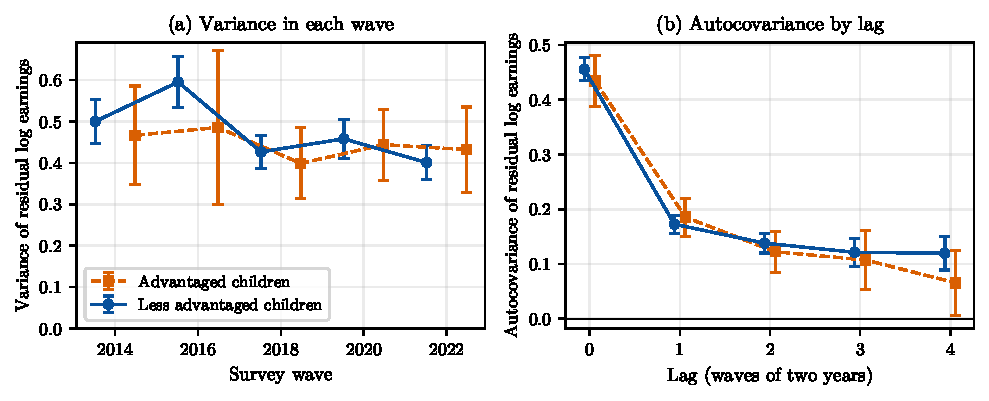
\includegraphics[width=0.86\textwidth]{figures/fig_autocov}
\caption{The second moments of residual log earnings by family background. Variance in each wave (panel a) and autocovariance by lag, averaged over waves (panel b), for advantaged and less advantaged children, with 95 percent bootstrap intervals (200 clustered replications). Residuals are demeaned within group and year (wave sizes 1,319, 1,049, 2,197, 2,083, and 2,001). Averages over waves weight each wave pair by the inverse of its
bootstrap variance. The two curves lie close together at lags zero to three and drift apart at lag four, with overlapping intervals at every lag; the longest lags are where the permanent--transitory split of
Table~\ref{tab:md} is decided.}
\label{fig:autocov}
\end{figure}

\begin{figure}[t]
\centering
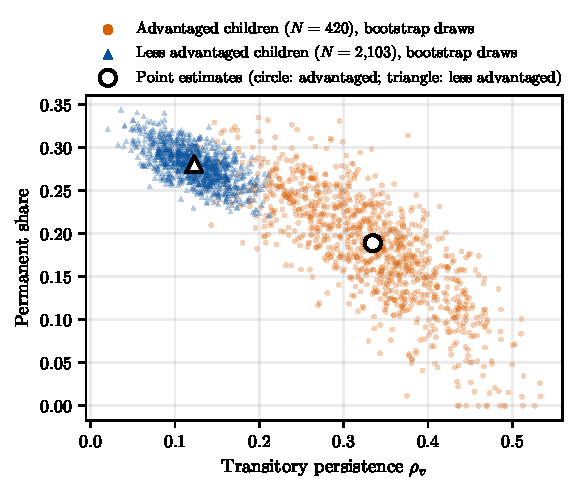
\includegraphics[width=0.50\textwidth]{figures/fig_ridge}
\caption{The identification ridge. Bootstrap draws and point estimates of the
fitted $(\rho_v, \text{permanent share})$ pair for advantaged and
less advantaged children, 1,000 clustered
replications of the cell-weighted estimator. The row of draws for advantaged children at a share of zero reflects the estimator's boundary constraint
($\sigma^2_\eta \ge 0$), not a separate mode.}
\label{fig:ridge}
\end{figure}

\subsection{Persistence by dynamic panel GMM}
\label{sec:abgmm}

A dynamic panel regression gives a second estimate of transitory
persistence. Residual earnings follow the autoregression
\begin{equation}
\tilde y_{it} = \rho_0\, \tilde y_{i,t-1}
 + \rho_1\, (\tilde y_{i,t-1} \times H_i) + \alpha_i + u_{it},
\label{eq:ab}
\end{equation}
in which the individual effect $\alpha_i$ absorbs the permanent
component, so the first-differenced estimator of
\citet{ArellanoBond1991}, with lagged levels as instruments, targets
the same transitory persistence as the minimum-distance fit; the
interaction lets persistence differ by parental occupation. Estimation is two-step GMM with cluster-robust two-step sandwich standard errors; the instruments are lags two and three, collapsed \citep{Roodman2009}. On the 2014--2022 panel the estimate for less advantaged children is
$\hat\rho_0 = 0.058$ (SE 0.036; Table~\ref{tab:ab}). The Hansen test does not
reject the moment set, and a test for second-order
serial correlation in the differenced residuals does not reject ($m_2$ $p = 0.50$). The reconstructed seven-wave panel gives 0.062, close to the five-wave figure, which is reassuring
about the income reconstruction. System GMM \citep{BlundellBond1998}, which adds level-equation
moments that are valid only under mean stationarity of initial
conditions, moves the point estimate to 0.109, and the Hansen test rejects the enlarged moment set ($p < 0.001$), so I keep the difference estimator.
The minimum-distance estimate for less advantaged children, 0.12, lies inside the 95 percent interval of the Arellano--Bond estimate, $[-0.01, 0.13]$.

Equation~\eqref{eq:rhoobs} sets
the two estimates of transitory persistence beside the autocorrelation that a regression without individual effects would deliver: with a permanent share near 0.27, the biennial autocorrelation of observed residual earnings implied by the minimum-distance fit is about $0.16 + 0.84 \times 0.27 \approx 0.39$ at one lag, more than twice the
minimum-distance estimate of the transitory parameter and further still
from the Arellano--Bond one. At the Arellano--Bond estimate, a shock that raises earnings by 10
percent in one wave raises them by about 0.6 percent in the next.

The interaction of lagged earnings with family background is imprecisely estimated, at 0.009 with a standard error of 0.094 and a Wald interval of $[-0.17, 0.19]$; inverting the
two-step overidentification test over a grid of imposed values gives a
set of $[-0.20, 0.29]$. The data exclude
large group differences in persistence but not moderate ones (the
smallest interaction the design detects with 80 percent power is 0.26),
and the point estimate gives no reason to think the groups differ.

\begin{table}[t]
\centering
\small
\caption{Arellano--Bond estimates of the persistence of transitory earnings shocks.}
\label{tab:ab}
\setlength{\tabcolsep}{3pt}
\begin{tabular}{@{}llcccc@{}}
\toprule
& & Less advantaged & Difference for & Hansen & \\
Panel & Estimator & children $\hat\rho_0$ & advantaged $\hat\rho_1$ & $J$ [$p$] & Instruments \\
\midrule
2014--2022 & Difference GMM & 0.058 & 0.009 & 2.38 & 4 \\
 &  & (0.036) & (0.094) & [0.304] &  \\
2014--2022 & System GMM & 0.109\rlap{***} & 0.055 & 20.86 & 6 \\
 &  & (0.034) & (0.092) & [0.000] &  \\
2010--2022 (reconstructed) & Difference GMM & 0.062\rlap{*} & $-0.043$ & 1.09 & 6 \\
 &  & (0.033) & (0.082) & [0.896] &  \\
\bottomrule
\end{tabular}

\par\smallskip
\begin{minipage}{0.92\textwidth}
\footnotesize\emph{Notes:} Two-step GMM, cluster-robust two-step sandwich standard errors in parentheses, clustered on child. The system row adds level equations instrumented by the collapsed lagged first difference. $N = 2{,}523$ children in the five-wave panel (2,272 usable differenced equations from 1,707 children); the reconstructed seven-wave panel applies the same screens to seven waves (2,776 equations from 1,839 children). Collapsed instruments, lags 2--3 (lags 2--4 on the seven-wave panel).
*, **, and *** denote significance at the 10, 5, and 1 percent levels; Hansen $J$ $p$-values in brackets.
\end{minipage}
\end{table}

\subsection{Nonlinear persistence and earnings growth}
\label{sec:abb}

Linear autoregressions average over a feature that
\citet{ArellanoBlundellBonhomme2017} document in American data: the
persistence of the earnings state depends on the worker's position in
the distribution and on the size of the shock. I fit their nonlinear
state equation $s_{it} = Q(s_{i,t-1}, U_{it})$, with $U_{it}$
uniform on the unit interval and $Q$ a sieve in Hermite polynomials
of the state (order two) and Bernstein polynomials of the shock rank
(order three), by stochastic EM on the 2014--2022 panel, and compute
the local persistence
$\rho(s, u) = \partial Q(s, u) / \partial s$. I use it
as a description. The fitted surface reproduces the American shape, with
strong persistence under middling shocks, more so higher in the
distribution, and large adverse shocks eroding high states. Persistence averaged uniformly over a $5 \times 5$ lattice of state
and shock-rank quantiles is 0.46 in the pooled sample, 0.54 for advantaged children, and 0.44 for less advantaged children; across ten runs of the stochastic estimator the pooled figure lies between 0.42 and 0.54, and the figure for advantaged children is the higher of the two in every run. The state in this model absorbs the permanent component, so its persistence is comparable to that of observed residual earnings in equation~\eqref{eq:rhoobs}, not to the transitory parameter.

Advantaged children might instead have steeper earnings paths. A fixed-effects regression of residual earnings on the interaction of the group indicator with a linear trend,
\begin{equation}
\tilde y_{it} = \alpha_i + \gamma\,(H_i \times t) + \delta' z_{it} + e_{it},
\label{eq:fe}
\end{equation}
where $z_{it}$ collects the time-varying covariates, gives $\hat\gamma = 0.018$ per wave (cluster SE 0.014) on the five-wave panel and 0.015 (SE 0.008) on the reconstructed panel without the covariates. The point estimates imply a divergence of 0.09 and 0.08 log points over a decade, and neither differs from zero at the 5 percent level. The strict-exogeneity restriction behind the fixed-effects
estimate is testable by adding the next observed wave's value of a
time-varying covariate \citep[Section~10.7.1]{Wooldridge2010}. Applied to
the urban indicator, the only substantive time-varying control, the
lead enters with coefficient 0.012 and a $t$-statistic of 0.23.

The absence of a growth gap does not conflict with the higher college completion of advantaged children. Children enter the panel at 31 on average. The least squares return to college is 0.37 at ages 26 to 29 and 0.46 at ages 30 to 34 (Section~\ref{sec:sample}), so for a child first observed at 31 most of the return is already in
the level of earnings, and the higher college completion of advantaged
children adds little to their measured growth. The cohorts born from
1989 onward, many of whom are first observed at ages 22 to 25, are the
exception.

\begin{table}[t]
\centering
\small
\caption{Group comparison across process moments.}
\label{tab:summary}
\begin{tabular}{@{}lccc@{}}
\toprule
Moment & Advantaged & Less advantaged & Gap \\
\midrule
All fifteen variances and autocovariances, joint test of equality & \multicolumn{2}{c}{---} & $p = 0.32$ \\
Fitted total variance (minimum distance) & 0.438 & 0.460 & $-0.022$ \\
Transitory persistence, Arellano--Bond & 0.066 & 0.058 & $+0.009$ \\
 &  &  & (0.094) \\
Nonlinear persistence, average over quantiles & 0.54 & 0.44 & $+0.11$ \\
Differential growth per wave, fixed effects & \multicolumn{2}{c}{---} & $+0.018$ \\
 &  &  & (0.014) \\
\addlinespace
\multicolumn{4}{@{}l}{\emph{Split of the common variance (weakly identified for advantaged children)}} \\
Permanent share (minimum distance) & 0.19 & 0.28 & $-0.09$ \\
 & (0.07) & (0.02) & (0.07) \\
Transitory persistence $\rho_v$ (minimum distance) & 0.33 & 0.12 & $+0.21$ \\
 & (0.08) & (0.03) & (0.08) \\
\bottomrule
\end{tabular}

\par\smallskip
\begin{minipage}{0.92\textwidth}
\footnotesize\emph{Notes:} Compiled from Tables~\ref{tab:md}--\ref{tab:ab} and Section~\ref{sec:abb}; the first row is the joint Wald test of Section~\ref{sec:md}. Standard errors in parentheses where available (the bootstrap of Table~\ref{tab:md} for the minimum-distance rows; the gap's standard error combines the two groups' standard errors). Gaps are computed from unrounded estimates.
\end{minipage}
\end{table}

\subsection{Reading the moments together}
\label{sec:together}

Table~\ref{tab:summary} collects the group comparison. Total variance,
the autocovariances, the dynamic panel autoregression, and average growth agree across the two groups. The fitted permanent--transitory split and the nonlinear state equation point the same way, toward shocks that fade more slowly for advantaged children, which is the opposite of protection; the split is weakly identified for
advantaged children, and the Arellano--Bond interaction, which targets the same persistence, is 0.009. Family
background is associated with the level of earnings, not with the variance of earnings around that level or with its growth, so whatever advantage these families confer must already be in the level; Sections~\ref{sec:premium} to \ref{sec:mediation} measure that level difference and ask how much of it is college.

Before turning to the level, I put the estimated process to a second use. Section~\ref{sec:measurement} asks how much a regression on a few waves of income understates the coefficient on permanent income; Section~\ref{sec:premium} uses the answer to compare two measures of parental income, and Section~\ref{sec:expansion} to weight averages of earnings.

\section{What the process implies for measurement}
\label{sec:measurement}

A regression that uses one year of income in place of permanent income
understates the coefficient. This section uses the estimated process to
say by how much, and how many waves of income are needed to undo most
of the bias. Let $y^*_i$ denote the permanent log income of the parents of child $i$
and suppose the researcher
observes $y_{iT} = y^*_i + \bar v_{iT}$, the average of $T$ waves of
parental income, which contains transitory variation. In a regression of a child
outcome on $y_{iT}$, the probability limit of the coefficient is the
true coefficient scaled by
\begin{equation}
\lambda_T \;=\; \frac{\sigma^2_\eta}
{\sigma^2_\eta + \sigma^2_\varepsilon / \big(T\,(1-\rho_v^2)\big)},
\label{eq:eta}
\end{equation}
treating the transitory components of the $T$ observed waves as mutually uncorrelated.\footnote{With biennial persistence $\rho_v = 0.16$ the exact variance of the $T$-wave average carries cross terms. The exact calculation, derived in Part II of the Online Appendix, lowers $\lambda_5$ from 0.65 to 0.59 and pushes the two-thirds crossing from six waves to eight, so the figures in the text, which use the simple formula, understate the attenuation.} Evaluated at the pooled estimates (panel A of Table~\ref{tab:eta}), the reliability ratio $\lambda_T$ is 0.27 at $T = 1$: a single wave recovers about a quarter of the coefficient on permanent income. Averaging helps quickly at first and slowly later. Recovering two thirds of the coefficient, about the share that \citet{Mazumder2005} finds short averages recover in the United States, takes about six biennial waves (eight under the exact calculation), a decade or more of panel coverage.

Transitory variation in a right-hand-side income measure attenuates the
coefficient by $\lambda_T$, whereas noise in the dependent variable costs
precision but not consistency. In a conventional intergenerational
elasticity regression the relevant $T$ is therefore the number of
parental income observations. A separate life-cycle correction applies
on top when income is observed far from mid-career
\citep{HaiderSolon2006}; the schedule here concerns panel length, not
observation age. The other case, noise in the dependent variable, arises in Section~\ref{sec:design}, where the outcome is an average of a child's own earnings over survey waves. The denominator of equation~\eqref{eq:eta} is the variance of such an average, and its inverse is the precision weight of the weighted expansion regression (equation~\eqref{eq:weights}).

\begin{table}[t]
\centering
\small
\caption{The attenuation schedule at the estimated parameters, and the raw estimates of \citet{FanYiZhang2021} corrected with it.}
\label{tab:eta}
\setlength{\tabcolsep}{3pt}
\begin{tabular*}{0.98\textwidth}{@{\extracolsep{\fill}}lccccccc@{}}
\toprule
\multicolumn{8}{@{}l}{\emph{A. Share of the coefficient on permanent income recovered by an average of $T$ waves}} \\
Waves averaged $T$ & 1 & 2 & 3 & 4 & 5 & 6 & 7 \\
\midrule
Reliability ratio $\lambda_T$, independence approximation & 0.27 & 0.43 & 0.53 & 0.60 & 0.65 & 0.69 & 0.72 \\
Reliability ratio $\lambda_T$, exact & 0.27 & 0.39 & 0.48 & 0.54 & 0.59 & 0.63 & 0.66 \\
Implied inflation factor $1/\lambda_T$ & 3.7 & 2.3 & 1.9 & 1.7 & 1.5 & 1.4 & 1.4 \\
\midrule
\end{tabular*}

\begin{tabular*}{0.98\textwidth}{@{\extracolsep{\fill}}lccc@{}}
\multicolumn{4}{@{}l}{\emph{B. Raw estimates of \citet{FanYiZhang2021} divided by the share recovered}} \\
Earnings process used for the correction & Share recovered & Implied coefficient & Authors' preferred \\
\midrule
Children's process (permanent share 0.27) & 0.39--0.54 & 0.31--0.45 & 0.390--0.442 \\
Linked parents' process (permanent share 0.43) & 0.59--0.74 & 0.22--0.30 & 0.390--0.442 \\
\bottomrule
\end{tabular*}
\par\smallskip
\begin{minipage}{0.98\textwidth}
\footnotesize\emph{Notes:} Panel A: equation~\eqref{eq:eta} at the pooled
estimates $\sigma^2_\eta = 0.125$, $\sigma^2_\varepsilon = 0.326$, $\rho_v = 0.16$. The exact row replaces the independence approximation
with the full variance of a $T$-wave average of serially correlated
transitory components. The inflation factor (for the approximation) is
what a researcher would multiply an estimated coefficient by to undo
attenuation, were the parameters known. Panel B: published raw least squares estimates,
0.166 for the cohort born 1970 to 1980 and 0.176 for the cohort born 1981 to 1988, with income averaged over two to four of the 2010 to 2016
waves. Share recovered is the fraction of a true coefficient that a
two-wave and a four-wave average recover under each process (exact
calculation; the transitory persistence of the linked parents is 0.02,
so for them the exact and the approximate schedules coincide). Implied coefficient is the published range divided by the
range of shares recovered. The authors' preferred estimates, one for each cohort, use income predicted from education and demographics and are not attenuated by design.
\end{minipage}
\end{table}

Panel B of Table~\ref{tab:eta} applies the schedule to a published
study that uses the same survey. \citet{FanYiZhang2021}
use its 2010 to 2016 waves, and their raw
least squares estimates of the intergenerational income elasticity, with income averaged over two to
four biennial waves, are 0.166 for the cohort born 1970 to 1980 and 0.176 for the cohort born 1981 to 1988. Dividing the smaller estimate by the largest share recovered and the
larger by the smallest implies a true coefficient between 0.31 and 0.45, an interval that contains their own preferred estimates for the two cohorts, 0.390 and 0.442,
which they obtain instead from income predicted by education and demographics with a
selection correction. The parent side can be checked directly, because
many linked parents are themselves panel respondents. The 542 linked parents aged 60 or younger with three or more waves of positive labor income have a permanent share of 0.43 (bootstrap interval $[0.35, 0.49]$) against 0.27 for the children, and a single wave of their income recovers a little over two fifths of the coefficient. Recomputing the shares recovered
at the parents' permanent share moves the implied coefficient to $[0.22, 0.30]$. Attenuation alone therefore closes between a quarter and just under one half of the distance from their raw estimates to their preferred
ones. The remainder is consistent with the life-cycle and selection
corrections their procedure performs beyond noise reduction.

The attenuation schedule describes incomes earned between 2014 and 2022. Parents
who earned under the administered wages of the urban sector in the
1980s and 1990s probably had a much smaller transitory share than the
three quarters I estimate for their children, and for studies that average their incomes
the schedule over-corrects. Rank-based
measures \citep{Chetty2014} reduce attenuation without removing it.
Simulation from the fitted process puts the single-wave recovery of the rank-rank slope at 0.52, roughly $\sqrt{\lambda_1}$, when the child's rank
is measured without error, and at 0.36 when the child's rank is measured from three waves, because rank noise
attenuates from both sides of the regression, unlike the levels case.

\section{The level premium}
\label{sec:premium}

Sections~\ref{sec:premium} to \ref{sec:mediation} study
the level of earnings defined in Section~\ref{sec:sample}. Of the 4,536 children in the sample, 2,774 (453
advantaged) have one. The others do not yet have two waves at the ages
over which it is measured; they enter only the regressions of
Section~\ref{sec:expansion}. The
premium is measured on this outcome because it is to be compared with the
return to college, which settles only at those ages. Before any controls, advantaged children earn 0.195 log points (22 percent) more than less advantaged children, and 34 percent of them completed college, compared with 14 percent.

\subsection{Estimand}
\label{sec:estimand}

The level premium is the association between $H_i$ and the child's level of
earnings, holding fixed the family income of the parental household and demographics. I leave two variables out of the regressions that measure the premium.
The first is parental education. In the parental cohorts of this sample, born mostly between the late 1930s and the early 1970s, schooling was interrupted and reallocated on
political criteria; the cohorts who would have entered college between 1966 and 1976 largely could not, and educational credentials were in large
part consequences of political and occupational position rather than
prior causes of it. If I controlled for parental education I would be
comparing parents in different occupations who have the same schooling \citep{AcharyaBlackwellSen2016, AngristPischke2009}.
In these cohorts two such parents are likely to differ in political
history, which I do not observe. The premium is therefore net of current family resources but not of every parental characteristic correlated with occupation, and it is an association rather than a causal effect. The second is the child's own education. Schooling is the
channel under investigation, and Sections~\ref{sec:expansion} and
\ref{sec:mediation} study it as a channel instead of removing it with a
control.

\subsection{Correlated random-effects estimates}
\label{sec:cre}

The main specification is a correlated random-effects (Mundlak)
regression \citep{Mundlak1978},
\begin{equation}
\log y_{it} \;=\; \delta_1 H_i \;+\; \delta_2\, \pinc_i \;+\; x_{it}'\gamma \;+\; \bar x_i'\xi \;+\; z_i'\kappa \;+\; \phi_t \;+\; \mu_p \;+\; u_{it},
\label{eq:cre}
\end{equation}
with $x_{it}$ the time-varying controls (age, urban status), $\bar x_i$
their within-child means, $z_i$ the time-invariant controls (gender), $\phi_t$ and $\mu_p$ year and province
effects, and clustering on person; $\delta_1$ estimates the premium
$\tau$. Before the parental income control enters, the occupation coefficient is 0.163 (SE 0.029).
Table~\ref{tab:cre} shows what conditioning on parental resources does
to it. Adding family income lowers the coefficient by nearly half, to 0.088 ($p = 0.002$). Replacing the family measure with the parents' own labor income, on the 2,185 children whose parents report it, moves
both coefficients in the direction that co-residence contamination
predicts: the income coefficient falls from 0.222 to 0.031 and the occupation coefficient rises to 0.153 ($p < 0.001$). The two columns err in opposite directions, so they bracket the premium. Column 1 over-controls, because family income contains the child's own earnings when the child lives with the parents. Column 2 under-controls: the parents' labor income leaves out asset and business income and is observed only in waves in which a parent works, 2.0 waves per parent on average compared with 5.6 for family income, so by the schedule of Section~\ref{sec:measurement} its coefficient is attenuated and it holds less of the family's resources fixed. The regression-based premium therefore lies between 0.088 and 0.153 log points (9 and 17 percent).

\begin{table}[t]
\centering
\small
\caption{The premium net of parental income: three estimates.}
\label{tab:cre}
\begin{tabular}{@{}>{\raggedright\arraybackslash}p{5.6cm}ccc@{}}
\toprule
& (1) & (2) & (3) \\
Estimator & Correlated & Correlated & Entropy \\
& random effects & random effects & balancing \\
Income control & Family income & Parental labor income & Family income \\
\midrule
\multirow[t]{2}{=}{Advantaged, $H$ (parent in CSCO 1--2 at child age 14)} & 0.088\rlap{***} & 0.153\rlap{***} & 0.072\rlap{**} \\
 & (0.029) & (0.034) & [0.01, 0.13] \\
\multirow[t]{2}{=}{Coefficient on parental income} & 0.222\rlap{***} & 0.031\rlap{***} & --- \\
 & (0.016) & (0.011) &  \\
Children & 2,774 & 2,185 & 2,774 \\
\bottomrule
\end{tabular}

\par\smallskip
\begin{minipage}{0.92\textwidth}
\footnotesize\emph{Notes:} Dependent variable: log annual labor income
by child and wave (columns 1 and 2) and the level of earnings (column
3). Columns 1 and 2: correlated random-effects regressions on the child-waves at ages 30 and over of the 2,774 children with a level of earnings (column 2: the 2,185 of them whose parents report labor income), standard errors clustered on person, controls for
age, year and province fixed effects, gender, urban status, and
within-child means of the time-varying covariates. Clustering at the family level instead changes the column 1 standard error by 0.0002 (159 of the 2,606 families have two or more of these children). Column 3: less advantaged children reweighted to match the first two
moments of parental income, gender, age, urban status, five-year birth cohort, and province (the fifteen largest separately) among advantaged children (equation~\eqref{eq:ebal}); the
bracket is a 200-replication bootstrap percentile interval.
*, **, and *** denote significance at the 10, 5, and 1 percent levels; the balancing estimate carries ** when its 95 percent bootstrap interval excludes zero.
\end{minipage}
\end{table}

\subsection{Entropy balancing}
\label{sec:ebal}

Entropy balancing \citep{Hainmueller2012} estimates the same premium by
a different route. It fits no earnings equation. Rather than matching each advantaged child to similar
less advantaged children, as propensity-score matching would, it reweights the whole
group of less advantaged children so that their weighted means and variances
of parental income, gender, age, urban status, five-year birth cohort, and province (the fifteen largest separately)
equal those of advantaged children exactly. The weights $w_i$ solve
\begin{equation}
\min_{w} \sum_{i:\, H_i = 0} w_i \log w_i
\quad\text{subject to}\quad
\sum_{i:\, H_i = 0} w_i\, g(x_i) = \frac{1}{N_1}\sum_{j:\, H_j = 1} g(x_j),
\quad \sum_{i:\, H_i = 0} w_i = 1,
\label{eq:ebal}
\end{equation}
where $g(x)$ collects the covariates and their squares and $N_1$ is the number of advantaged children; the weights stay as
close as possible to uniform weights while balancing the moments, and
the premium is the difference between the advantaged mean of log
earnings and the weighted mean of less advantaged children. The balanced difference in mean log
earnings is 0.072, or 7 percent, with a 200-replication bootstrap percentile interval of $[0.01, 0.13]$. Under the same weights the
gap in college completion between the groups is 0.122, or 12.2 percentage points (33.55 percent of advantaged children against 21.30 percent of reweighted less advantaged children; interval $[0.08, 0.17]$). Section~\ref{sec:mediation} converts this gap into earnings. Both figures are for all 2,774 children, the cohorts before and after the reform together. Regression and balancing condition on the
same observables, and with the same income measure they give nearly the
same premium, 0.088 and 0.072. Neither can speak to unobserved
confounding.

\subsection{Competing markers of social position}
\label{sec:class}

If the occupation indicator proxies for social position broadly, then other
markers of position should add little once it enters. The Chinese
setting supplies two natural competitors: party membership, which has its own literature on labor-market premia \citep{LiEtAl2007}, and employment inside the state system. Both are concentrated among the parents the indicator picks out. Parental party
status when the child was fourteen comes from the same retrospective
battery as the occupation question; 45 percent of advantaged children had a parent who was a party member, compared with 15 percent of less advantaged children.
State-sector employment is proxied by the linked parents' work-unit
category in 2012, available for the 34 percent of children with a
parent still working then; among them, 42 percent of advantaged children have a parent in the state sector, compared with 17 percent of less advantaged children. Table~\ref{tab:markers} enters each marker
with and without the occupation indicator in regressions of the level of earnings, one observation per child, with parental income and the controls listed in the table notes.

On its own, party membership carries a coefficient of 0.042 and
state-sector employment one of 0.048 (columns 2 and 5), a little over half of the
occupation coefficient on the same children (0.076 and 0.083), and
neither is distinguishable from zero. Once parental occupation enters (columns 3 and 6), the
party coefficient falls to 0.026 and the state-sector coefficient to 0.035,
while the occupation coefficient barely moves, to 0.070 and 0.077. Neither marker adds detectably to parental occupation: the 95 percent intervals of the conditional
coefficients reach 0.08 for party membership and 0.12 for
state-sector employment (8 and 13 percent), which bounds any independent effect of either marker. The pattern fits the institutions of the parents' working years: a post in government, enterprise management, or the professions was usually a post inside the state system, and party membership was a common step on the career that led to it, so parental occupation already records what the two other markers measure.

\begin{table}[t]
\centering
\small
\caption{Party membership and state-sector employment as competing markers.}
\label{tab:markers}
\setlength{\tabcolsep}{6pt}
\begin{tabular}{@{}lcccccc@{}}
\toprule
& \multicolumn{3}{c}{Parental party membership} & \multicolumn{3}{c}{Parental state-sector} \\
& \multicolumn{3}{c}{when the child was fourteen} & \multicolumn{3}{c}{employment in 2012} \\
\cmidrule(lr){2-4}\cmidrule(lr){5-7}
& (1) & (2) & (3) & (4) & (5) & (6) \\
\midrule
Advantaged, $H$ & 0.076\rlap{***} &  & 0.070\rlap{**} & 0.083\rlap{*} &  & 0.077 \\
 & (0.030) &  & (0.031) & (0.047) &  & (0.048) \\
Party membership &  & 0.042 & 0.026 &  &  &  \\
 &  & (0.026) & (0.027) &  &  &  \\
State-sector employment &  &  &  &  & 0.048 & 0.035 \\
 &  &  &  &  & (0.045) & (0.046) \\
\addlinespace
Children & 2,766 & 2,766 & 2,766 & 937 & 937 & 937 \\
\bottomrule
\end{tabular}

\par\smallskip
\begin{minipage}{0.9\textwidth}
\footnotesize\emph{Notes:} Each column is one regression of the level of earnings (mean log labor income net of survey-year effects over the waves at ages 30 and over) on the regressors shown, one observation per child. Controls: parental income,
gender, urban residence, age at first observation and its square, and
province effects. Heteroskedasticity-robust standard errors in parentheses. Columns 1 to 3: children with a report of parental party membership (8 children lack one); party membership is either parent a member of the Communist
Party, a democratic party, or the Youth League when the child was
fourteen (retrospective report). Columns 4 to 6: children with a parent working in 2012; state-sector employment is either linked
parent working in a government, party, or military unit, a public
institution, or a state-owned enterprise in that year.
*, **, and *** denote significance at the 10, 5, and 1 percent levels.
\end{minipage}
\end{table}

\begin{figure}[t]
\centering
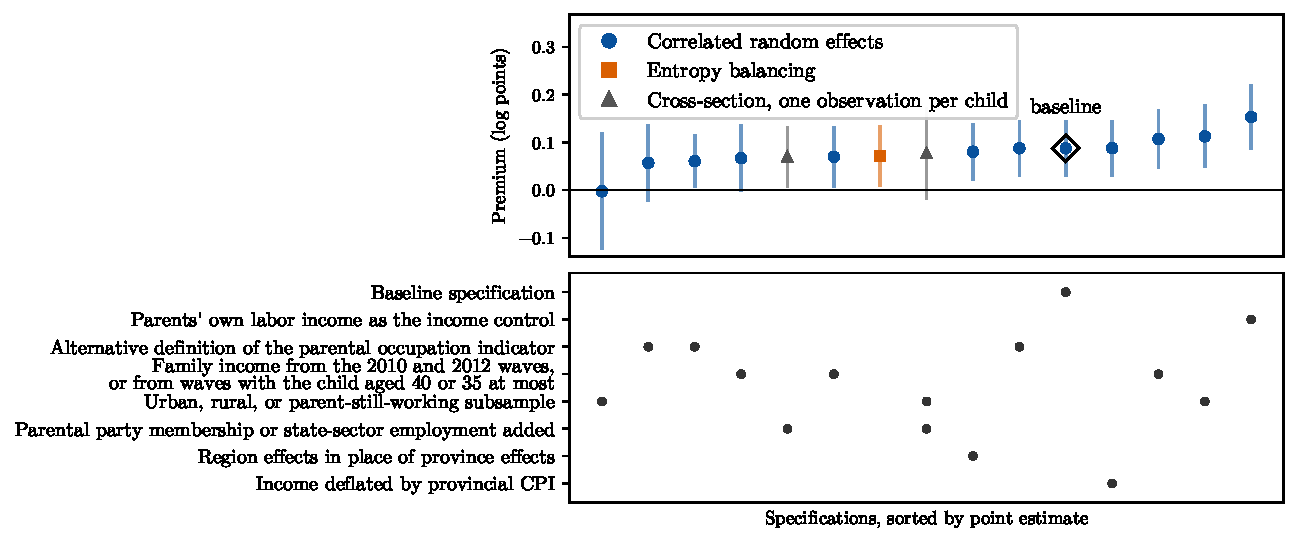
\includegraphics[width=0.92\textwidth]{figures/fig_spec_curve}
\caption{The premium in fifteen specifications. The premium is the earnings gap between advantaged and less advantaged children with parental income held fixed; specifications are sorted by point estimate. Vertical bars are 95
percent confidence intervals; the diamond marks the baseline; the lower
panel marks the analytic choices in each specification.}
\label{fig:spec}
\end{figure}

\subsection{Robustness of the premium}
\label{sec:premrobust}

Figure~\ref{fig:spec} arranges fifteen specifications in a single
sorted plot with the analytic choices marked underneath. They vary the income control (the parents' own labor income; family income from the 2010 and 2012 waves only, which precede the earnings window; family income from the waves in which the child was at most 40 or at most 35) and the definition of the indicator (the most frequent retrospective report, which classifies every child as the baseline does; CSCO group 3 added; group 1 alone). They also vary the estimator (entropy balancing; the regressions of Section~\ref{sec:class} with a competing marker added), the province effects and the deflator, and the subsample (children recorded as urban or as rural in most of their waves; the specification with state-sector employment uses the children with a parent working in 2012). The estimates run
from $-0.002$ (children recorded as rural in most waves) to 0.153 (the
parents' own labor income as the income control); ten of the fifteen lie between 0.06 and 0.09, and eleven intervals exclude zero. The Online Appendix lists all fifteen.

The retrospective indicator and the indicator based on current
occupations disagree for 14 percent of the children in the sample for whom both exist (15 percent among those with a level of earnings). By the result of \citet{Bollinger1996} for a misclassified binary
regressor, misclassification unrelated to the child's outcome and to the controls can only have shrunk the premium; under
that assumption 0.088 is a lower bound. With the indicator based on current occupations, measured after the formative years, the estimate is 0.049 ($p = 0.27$); it is not among the fifteen.

\section{The college channel: the 1999 expansion}
\label{sec:expansion}

\subsection{The reform and provincial intensity}
\label{sec:background}

Section~\ref{sec:premium} measured the premium; this section and the next ask how much of it runs through college. I use the 1999 expansion to learn which children the added seats admitted and what college returned to them. Through the 1990s, admission to Chinese universities was rationed by score on the national college entrance examination under a centrally planned enrollment quota that grew slowly, from roughly 0.7 million admissions in 1988 to one million in 1997, while candidates far outnumbered seats. For most students the binding constraint was the number of seats rather than the willingness to take the examination. The cost of competing for a seat also varied with family circumstance: opportunity costs
were high even where tuition was low, provincial admission cutoffs
differed, and urban schools prepared students better for the
examination.

In June 1999, after registration for that year's entrance examination
had closed, the central government announced a second and larger increase in that year's admissions \citep{LiWhalleyXing2014}; admissions grew by more than 40 percent in 1999 and passed five million by 2005. The trigger was
macroeconomic as much as educational, and the proposal moved from
memorandum to decision within months. Provinces had little time to fit seats to local demand for skill, and seats grew where existing institutions could add
them, on a timetable set in Beijing. The placebo instrument defined below, built from pre-reform growth in examination registrations, has no first stage (Table~\ref{tab:mature}), which is consistent with this account.

By 1997 every institution charged tuition \citep{DongWan2012}, so the reform relaxed the seat
constraint while prices stayed positive, and the marginal student it
admitted had to clear a resource bar as well as the examination bar.
Admission operated through provincial quotas set institution by
institution, and a national percentage increase translated into different
seat growth across provinces depending on where seats could
be added; that administrative fact is the source of the cross-province
variation the design uses. The intensity measure defined below accordingly counts the
seats that institutions located in a province added, not the seats
allotted to the province's own candidates. The two nearly coincide:
institutions set their admission plans province by province and
reserve the largest share for the province in which they are located,
so a child, who takes the examination in the home province, competes
mainly for the seats of that province's institutions. The expansion grew the four-year (\emph{benke}) and three-year (\emph{dazhuan}) tiers of higher education at different provincial rates; college completion throughout means sixteen or more
years of schooling, the four-year degree.

Children born in 1981 or later reached age eighteen in the expansion
era. The 1981 cohort was admitted under the enlarged quota without
having planned for it, because registration for 1999 had closed before
the announcement; the first cohort able to plan around the policy took
the examination in 2000. The cohort dimension of the instrument is the
ratio of actual national admissions in the year a cohort turned
eighteen to a linear projection of the pre-reform trend, both computed from the national admissions series in \citet{Ma2024IER}. The ratio lies between 0.9 and 1.6 for the cohorts born 1964 to 1976 and between 1.02 and 1.05 for those born 1977 to 1980, rises to 1.44 for the 1981 cohort, and reaches 4 for the cohorts born around 1990. Exposure enters
continuously, and the birth-year effects of the specification absorb
the level break together with every other common cohort movement.

Provincial intensity follows \citet{Ma2024IER}. The main measure is the
number of college graduates of 2006 to 2010 that the province's institutions are predicted to produce, divided by the province's
stock of college-educated workers in 2005. The prediction allots the national number of graduates to cities by their shares of national college enrollment in the 1982 census, because the expansion scaled up the institutions that already existed, and counts graduates where they studied. Two other normalizations of the same predicted inflow, by total employment in 2005 and as the log of the implied growth of the college-educated stock, serve as checks.
The enrollment shares were fixed long before the reform, but the denominators are measured in 2005, after it had begun. The analysis therefore also uses a
measure that is predetermined in every component, the census share of each province's
adults born 1956 to 1976 who had completed senior secondary school. The
share describes the size of the province's education system before the
reform, was fixed at least five years before it, is stable
across censuses (correlation 0.97 between the 1990 and 2000
measurements), and correlates 0.44 with the main measure across provinces. Statistical yearbooks supply a placebo.
The growth of college entrance examination (CEE) registrations before
the reform,
$\log(\mathrm{CEE}_{1998,p} / \mathrm{CEE}_{1997,p})$, is upstream of
admissions and predetermined. Interacted with cohort exposure, it should not predict college completion if the design isolates the reform rather than generic provincial trends.\footnote{Provincial registration counts come from the annual \emph{Chinese Educational Statistical Yearbook} through the CNKI statistical-data platform. The 1997 total for Inner Mongolia in the source export disagrees with adjacent years and with the counts of men and women printed beside it, and is replaced by their sum, 66{,}674.}

\subsection{Design and threats}
\label{sec:design}

The design, in the tradition of \citet{Duflo2001}, instruments college completion $M_i$ (sixteen or more years
of schooling) with provincial intensity multiplied by cohort exposure,
$Z_i = \mathrm{Intensity}_{p(i)} \times \mathrm{Exposure}_{c(i)}$. The outcome is the level of earnings (Section~\ref{sec:sample}). The conventional regression has one observation for each of the 2,774 children who have a level of earnings, $\bar y_{io}$ (the subscript $o$ marks earnings at ages 30 and over):
\begin{equation}
\begin{aligned}
\bar y_{io} &= \beta_o M_i + \theta_1 H_i + \delta' X_i + \mu_{p(i)} + \mu_{c(i)} + e_{i}, \\
M_i &= \pi_o Z_i + \psi_1 H_i + \gamma' X_i + \mu_{p(i)} + \mu_{c(i)} + u_i,
\end{aligned}
\label{eq:oldonly}
\end{equation}
where $X_i$ contains $\pinc_i$, gender, and urban residence, $\mu_{p(i)}$ are province
effects, and $\mu_{c(i)}$ is one effect per birth year. The coefficient $\beta_o$ is the return to college in the level of earnings, and $\pi_o$ is its first-stage coefficient.

The main specification adds a second row to this regression. Equation~\eqref{eq:oldonly} leaves
out the 1,762 children in the sample who are not yet 30 or have fewer
than two waves at 30 and over, although they belong to the same
provinces and birth cohorts and carry information on the province effects, the birth-year effects, and the coefficients on the controls. The gain is largest for the estimates by family background, in which birth-year effects are specific to each group: the added rows bring 302 more advantaged children into the estimation of those effects. I therefore give each child up to two rows. The row at 30 and over holds $\bar y_{io}$, a mean over at least two waves because transitory variance is three quarters of the variance of
earnings in a single wave (Section~\ref{sec:measurement}). The row below 30 holds $\bar y_{ib}$, the
same mean over the child's waves at ages 22 to 29, and exists when the
child has at least one such wave. The 4,536 children contribute 2,774
rows at 30 and over and 2,343 rows below 30; 581 children contribute
both. Let $r \in \{o, b\}$ index the rows of child $i$ and let $O_r$
equal one for the row at 30 and over. The two-row specification is
\begin{align}
\bar y_{ir} &= \beta_o\, M_i O_r + \beta_b\, M_i (1 - O_r) + \theta_1 H_i
+ \theta_2 H_i O_r + \theta_3 O_r + \delta' X_i + \mu_{p(i)} + \mu_{c(i)} +
e_{ir}, \label{eq:twoband} \\
M_i O_r &= \pi_o\, Z_i O_r + \pi_{b}\, Z_i (1 - O_r) + \psi_1 H_i
+ \psi_2 H_i O_r + \psi_3 O_r + \gamma' X_i + \mu_{p(i)} + \mu_{c(i)} +
u_{ir}. \label{eq:fso}
\end{align}
College completion enters equation~\eqref{eq:twoband} separately for the two rows, and each of the two terms has its own instrument: $M_i O_r$ is instrumented by $Z_i O_r$ and $M_i (1 - O_r)$ by $Z_i (1 - O_r)$. Equation~\eqref{eq:fso} is the first stage for $M_i O_r$; the one for $M_i (1 - O_r)$ has the same form. $\theta_3$ lets mean earnings differ between
the rows and $\theta_2$ lets the premium differ between them; the province effects, the birth-year effects, and the coefficients on $X_i$ are common to the two rows.

Three coefficients carry the results: the return $\beta_o$, its first-stage coefficient $\pi_o$, and its reduced form, the coefficient on $Z_i O_r$ in the regression of $\bar y_{ir}$ on the two instruments and the controls. As in equation~\eqref{eq:oldonly}, $\beta_o$ is the return to college in the level of earnings, and the conventional regression gives nearly the same value (0.70 against 0.68, Section~\ref{sec:earnings}). I do not report or interpret $\beta_b$: every child observed below 30 between 2014 and 2022 was born in
1985 or later and reached college age well after the expansion had begun, so the reform does not identify it.

Two variants show what the second row and the equal weighting of rows
contribute. The first is the conventional regression of equation~\eqref{eq:oldonly}.
The second keeps both rows and weights them. The rows are means of
different numbers of waves, and the earnings process of
Section~\ref{sec:process} says how much noisier a mean of few waves is.
Under equation~\eqref{eq:feAR}, with the transitory components of a
child's waves treated as uncorrelated as in equation~\eqref{eq:eta},
the mean of $n_{ir}$ waves has variance
$\sigma^2_\eta + \sigma^2_v / n_{ir}$, where
$\sigma^2_v = \sigma^2_\varepsilon / (1 - \rho_v^2)$. This variance is the denominator of equation~\eqref{eq:eta} with $n_{ir}$ in place of $T$, and the weight of
a row is its inverse,
\begin{equation}
w_{ir} \;=\; \left( \hat\sigma^2_\eta +
\frac{\hat\sigma^2_\varepsilon}{(1 - \hat\rho_v^2)\, n_{ir}}
\right)^{-1},
\label{eq:weights}
\end{equation}
evaluated at the pooled estimates of Table~\ref{tab:md} ($\hat\sigma^2_\eta = 0.125$, $\hat\sigma^2_\varepsilon = 0.326$, $\hat\rho_v = 0.16$). A row that averages one wave has weight 2.2 and a row that averages five waves 5.2. The same three parameters do two jobs. In Section~\ref{sec:measurement} they say how much a noisy regressor attenuates a coefficient; here they say how precisely an average of earnings measures an outcome. I keep the unweighted regression as the main specification because it does not depend on the fitted process, and Section~\ref{sec:earnings} reports the
weighted one beside it.

Each child is assigned the province of residence in the first
wave in which the child is observed at ages 22 to 55, and the birth year that wave implies. The province is a
proxy for the province of examination registration, since CFPS does not
record hukou province at age eighteen. A child who moved before that wave for reasons
unrelated to schooling is assigned the wrong intensity, which attenuates
provincial contrasts. Such moves are uncommon and no more common in one group than in the other: of the 2,578 children for whom the 2010 wave records the province of residence at age twelve, 8 percent of advantaged children and 7 percent of less advantaged children are assigned a different province. Section~\ref{sec:earnings} reports the estimates with the instrument
assigned by the province at age twelve.

The model is exactly identified, with one excluded instrument
for each endogenous regressor, and
two-stage least squares and LIML coincide. Intensity varies at
the province level, so inference rests on 29 clusters. I
report wild cluster bootstrap $p$-values \citep[Rademacher weights by
province, null imposed, 9,999 replications;][]{CameronGelbachMiller2008} and wild-cluster
Anderson--Rubin sets for the instrumented returns to college; the sets remain valid when the first stage is weak, and both are more reliable than cluster-robust asymptotics with so few clusters. Randomization inference requires no large-cluster approximation. I reassign the 29 provincial values of intensity at random among the provinces 4,999 times, holding every child's cohort exposure, outcomes, and controls fixed. No reassignment yields an earnings reduced-form $t$-statistic as large in absolute value as the actual one, and two yield a first-stage $t$-statistic as large ($p < 0.001$ for both). Reassigning intensity only among the provinces of the same region (east, center, and west) again gives $p < 0.001$ for both. The
two rows of a child lie in the same province, so clustering on province
allows for their correlation.

First-stage strength is reported as the
cluster-robust $F$ on $Z_i O_r$ in equation~\eqref{eq:fso}, the one instrument that is not zero on the rows at 30 and over; in the
conventional regression of equation~\eqref{eq:oldonly}, which has one instrument and one
endogenous regressor, the same statistic equals the effective $F$ statistic of
\citet{OleaPflueger2013}. Birth-year effects absorb the national path of admissions, which is 86 percent of the instrument's variance net of province effects; the estimates rest on the remaining 14 percent, the interaction of provincial intensity with cohort exposure.

Identification is that of an exposure design, the exogenous-shares case of
\citet{GoldsmithPinkham2020} with provincial intensity as the single share and cohort exposure as the shift: provincial intensity must be unrelated to
province-by-cohort shocks to the outcomes, conditional on province and
cohort means. Province fixed effects absorb any time-invariant relation
between intensity and outcome levels (high-intensity provinces are
richer on average), so the remaining threats are trending confounders.
Provinces with rapid pre-reform growth in examination demand might be
on differential trends more generally; if so, an intensity measure built from pre-reform registration growth should generate a spurious first stage, and none appears ($F = 0.5$ against 18.0). The first stage follows where seats were added, not where examination demand had been growing before the reform.

Exclusion requires that the instrument move the outcomes only through
college, conditional on the controls; the main
competing shock of the period is WTO accession, whose provincial
geography could correlate with provincial intensity. The expansion also enlarged the supply of graduates, which lowered the relative wages of graduates in the cohorts entering the labor market \citep{KnightDengLi2017}; to the extent that graduates work where they studied, their lower relative wages push the earnings reduced form toward zero. Table~\ref{tab:threats} lists each assumption with its main threat, the checks I run, and their results (Sections~\ref{sec:earnings} and \ref{sec:occupation}).

\begin{table}[t]
\centering
\footnotesize
\caption{Identifying assumptions, threats, and diagnostics.}
\label{tab:threats}
\begin{tabular}{@{}L{2.8cm}L{3.9cm}L{8.0cm}@{}}
\toprule
Assumption & Principal threat & Diagnostic and result \\
\midrule
Instrument relevance & Weak first stage in a group or under another intensity measure
& First-stage $F$ of 18.0 for all children, 16.9 and 12.3 by family background, and 13.3 to 39.8 under the three other measures (Tables~\ref{tab:mature} and \ref{tab:groups}) \\
\addlinespace
Exclusion: the instrument reaches earnings only through college & A shock of the reform years, such as trade after WTO accession, that is correlated with intensity and reaches earnings outside college &
Trade-exposure controls: reduced form 0.127 to 0.140, against 0.128. Children with nine or fewer years of schooling: occupation 0.017 (SE 0.019). Reduced form of the child's adult urban residence: 0.006 (SE 0.022) \\
\addlinespace
Parallel trends: provincial intensity unrelated to province-by-cohort shocks & Provinces that added more seats were already on different trends &
Placebo from pre-reform registration growth: first-stage $F$ of 0.5. Predetermined census measure: return 0.67. Cohorts born in 1980 or earlier: no trend in earnings or completion ($p = 0.56$ and $0.75$). Linear cohort trends by region: return 0.72. Census cohorts before the reform: under one percentage point of divergence over 20 cohorts \\
\bottomrule
\end{tabular}
\end{table}

\subsection{First stages and whom the reform moved}
\label{sec:firststage}

Panel (a) of Figure~\ref{fig:fs} plots the college completion
rate by family background in five groups of birth cohorts.
Advantaged children complete college at a rate of 17.3 percent in the pre-reform cohorts and 50.5 percent in the post-reform cohorts; less advantaged children
start at 4.6 percent and reach 24.2. Completion rose in both groups,
by about 33 percentage points among advantaged children and by 20 among
less advantaged children, so the gap widened from 13 to 26 percentage points while the ratio of the two completion rates fell from 3.7 to 2.1. By group of cohorts, the ratio printed under each group in the figure falls from 6.1 in the cohorts
born in 1972 or earlier to 1.9 in those born 1989 to 1997. Panel (b)
shows the first stage of each group as a binned scatter (20 bins of
less advantaged and 10 bins of advantaged children, with equal numbers
of children), in the specification described below.

\begin{figure}[t]
\centering
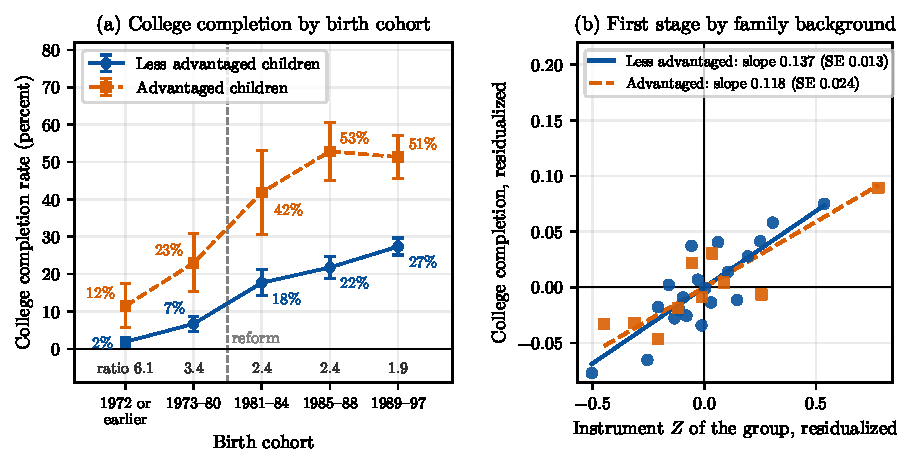
\includegraphics[width=0.92\textwidth]{figures/fig_first_stage}
\caption{College completion by family background and the first stage. Panel (a): college completion rate by family background in five groups of birth cohorts, with 95 percent intervals; the number under each group is
the ratio of the rate of advantaged children to the rate of less
advantaged children. Panel (b): binned scatter of
college completion on the instrument by family background, in the
regression with province effects common to the two groups and
birth-year effects specific to each; both variables are residualized on
the other group's instrument and the controls, and the lines have the group first-stage slopes with province-clustered standard errors. All 4,536 children in the sample, one observation per child.}
\label{fig:fs}
\end{figure}

On all 4,536 children, one observation per child, the main intensity
measure delivers a first-stage coefficient of 0.136 (SE 0.013) with
$F = 102.9$, and the three other measures give first-stage $F$
statistics between 14 and 68 (Table~\ref{tab:mature}). Relative to the cohorts born before 1981, moving from a
province at the 25th percentile of intensity to one at the 75th raises
the college completion of a cohort born in 1989 or later by 8 percentage points. The first stage that the returns of Section~\ref{sec:earnings}
rest on is $\hat\pi_o$ of equation~\eqref{eq:fso}, the one for the rows at 30 and over: 0.186 (SE 0.044) with $F = 18.0$. It is weaker than the
first stage on all children because it rests on the 2,774 children
already observed at those ages, of whom 1,444 were born in 1981 or later.

To estimate the first stage by family background I
let the instrument enter separately for the two groups in one
regression. Birth-year effects are specific to each group, so each
group's national rise in completion is removed separately. Only 453 advantaged children have a level of earnings, fewer than 20 in 23 of the 29 provinces. That is too few to
estimate a separate set of province effects for them, so I make province effects common to the two groups. On all
children the first-stage coefficient is 0.137 (SE 0.013,
$F = 114.3$) for less advantaged children and 0.118 (SE 0.024,
$F = 24.1$) for advantaged children, and the difference between them,
$-0.019$ (SE 0.019), is not distinguishable from zero. Added seats raised completion in the two groups by a similar number of percentage points (8 and 7 for the same interquartile difference). Relative to pre-reform rates of 4.6 and 17.3 percent, the response of less advantaged children is four times as large.

Fees had been in place since 1997, yet completion among less
advantaged children was five times as high in the cohorts after the reform as in those before it, and it rose more where more seats were added. A lower cutoff admitted children who had been below the old one, as both readings in the introduction imply. The readings differ in the return these children earned, which Section~\ref{sec:earnings} estimates.

\subsection{Earnings}
\label{sec:earnings}

The premium is a gap in earnings, so what Section~\ref{sec:mediation} needs is the effect of college on the earnings of the children the expansion admitted. The specification is the two-row regression of
equation~\eqref{eq:twoband}, and, unless noted, every estimate below is the one for the row at 30 and over; the cohorts born before 1981 supply the earnings
gradient on provincial intensity in the absence of the reform.

\begin{table}[t]
\centering
\small
\caption{Earnings and occupation: first stages, reduced forms, and instrumented returns across measures of provincial intensity.}
\label{tab:mature}
\setlength{\tabcolsep}{4pt}
\begin{tabular}{@{}>{\raggedright\arraybackslash}p{4.0cm}ccccc@{}}
\toprule
& \multicolumn{2}{c}{First-stage $F$} & & & \\
\cmidrule(lr){2-3}
& Rows at 30 & One observation & Earnings & Instrumented & Occupation \\
Intensity & and over & per child & reduced form & return & reduced form \\
\midrule
\multirow[t]{3}{=}{Predicted inflow per 2005 college-educated worker (main measure)} & 18.0 & 102.9 & 0.128\rlap{***} & 0.68 & 0.092\rlap{**} \\
 &  &  & (0.018) & $[0.50, 4.20]$ & (0.026) \\
 &  &  & [0.002] &  & [0.016] \\
\addlinespace
\multirow[t]{3}{=}{Predicted inflow per 2005 worker} & 39.8 & 51.2 & 0.454\rlap{**} & 0.63 & 0.274\rlap{*} \\
 &  &  & (0.054) &  & (0.087) \\
 &  &  & [0.017] &  & [0.080] \\
\addlinespace
\multirow[t]{3}{=}{Log implied growth of the college-educated stock} & 13.3 & 68.4 & 0.204\rlap{***} & 0.72 & 0.150\rlap{**} \\
 &  &  & (0.032) &  & (0.039) \\
 &  &  & [0.002] &  & [0.010] \\
\addlinespace
\multirow[t]{3}{=}{Census share with senior secondary} & 16.8 & 13.7 & 0.294\rlap{*} & 0.67 & 0.156\rlap{**} \\
 &  &  & (0.060) &  & (0.046) \\
 &  &  & [0.051] &  & [0.029] \\
\addlinespace
\multirow[t]{3}{=}{Pre-reform registration growth 1998/1997 (placebo)} & 0.5 & 0.0 & $-0.010$ & --- & --- \\
 &  &  & (0.077) &  &  \\
 &  &  & [0.893] &  &  \\
\bottomrule
\end{tabular}

\par\smallskip
\begin{minipage}{0.92\textwidth}
\footnotesize\emph{Notes:} All 4,536 children in the sample (755 advantaged), two-row specification of equation~\eqref{eq:twoband}; every entry except the column headed One observation per child is the estimate for the row at 30 and over (2,774 rows, of which 1,444 belong to children born in 1981
or later). That column is the first-stage $F$ of the regression of college completion on the instrument with one observation per child (4,536 children) and the controls of equation~\eqref{eq:oldonly}. Dependent variables: the level of earnings; the share of the child's waves at those ages in which the reported occupation is official, managerial, or professional (CSCO major groups 1--2). Province-clustered standard errors in parentheses and
wild cluster bootstrap $p$-values in brackets (9,999 Rademacher
replications by province, null imposed). The instrumented return is the two-stage least squares estimate of $\beta_o$, and the bracket under the return in the first row is its 95 percent wild-cluster Anderson--Rubin set. Reduced forms are per unit of each measure and are not comparable across rows. The last column is the reduced form of the occupation share on the instrument; the instrumented effect of college on that share under the main measure is 0.50.
*, **, and *** denote significance at the 10, 5, and 1 percent levels according to the wild cluster bootstrap $p$-values.
\end{minipage}
\end{table}

In Table~\ref{tab:mature}, the first stage $\hat\pi_o$ of Section~\ref{sec:firststage} has $F = 18.0$ (wild-cluster $p = 0.03$) and the earnings reduced form is 0.128 (SE
0.018, wild-cluster $p = 0.002$): an interquartile difference in intensity (0.59 in $Z$, which on the rows at 30 and over raises completion by 11 percentage points) raises the level of earnings of a cohort born in 1989 or later by about 0.076 log points (8 percent). The two-stage least squares estimate of the return to college is 0.68 log points, against a least squares return of 0.45. The 95 percent wild-cluster Anderson--Rubin set is $[0.50, 4.20]$: it excludes zero and the least squares return. Inverting the randomization test under a common return, with reassignment within regions, gives a narrower 95 percent set, $[0.45, 1.30]$.

The three other intensity measures give
returns of 0.63 to 0.72 with wild-cluster $p$ between 0.002 and 0.051,
and the placebo intensity does not predict completion ($F = 0.5$). Children
with nine or fewer years of schooling, who were never candidates for
college, did not respond: the share of their working years spent in official, managerial, or professional occupations has a reduced form of 0.017 (SE 0.019), against 0.092 for all children (Section~\ref{sec:occupation}). The trade-exposure controls of Table~\ref{tab:threats}, cohort exposure interacted with a coastal indicator and with the province's export share, leave the reduced form at 0.127 to 0.140, and dropping one province at a time gives returns between 0.65 and 1.11. The child's urban residence in adulthood, a route to higher earnings outside college, does not move with the instrument (reduced form 0.006, SE 0.022, one observation per child).

Figure~\ref{fig:mature} reports the event study. With the cohorts born 1977 to 1980 as reference, the earnings gradient on provincial intensity, in log points per unit of intensity, is $-0.03$ and 0.01 in the two pre-reform bins and rises to 0.12, 0.25, and 0.60 for the cohorts born 1981 to 1984, 1985 to 1988, and 1989 or later. The completion gradient is $-0.02$ and 0.21 in the two pre-reform bins, neither distinguishable from zero at the 5 percent level, and 0.25, 0.50, and 0.65 in the three post-reform bins, where it rises with the exposure of the cohort.

\begin{figure}[t]
\centering
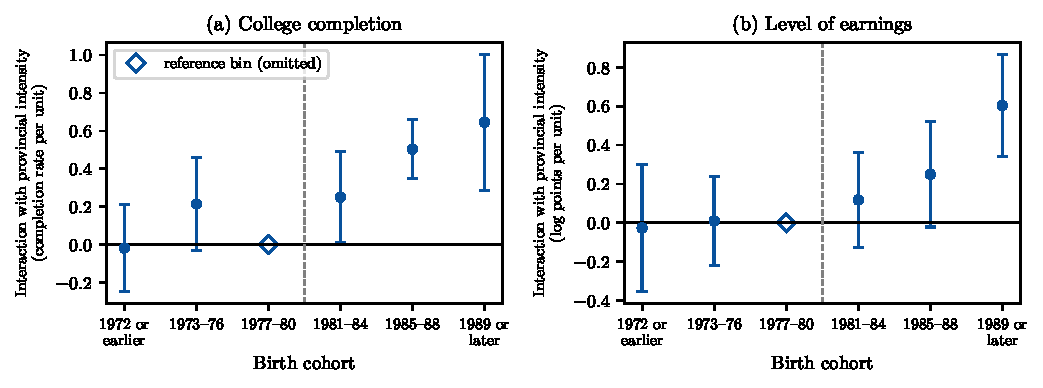
\includegraphics[width=0.92\textwidth]{figures/fig_mature_age}
\caption{Event study. College completion (panel a) and the level of earnings (panel b) by cohort bin: coefficients on
interactions of provincial intensity with the birth-cohort bins
1972 or earlier, 1973--1976, 1981--1984, 1985--1988, and 1989 or later, with the reference bin 1977--1980 plotted at zero. Main intensity measure; the 2,774 children with a level of earnings; demographic controls, birth-year effects, and province effects included; 95 percent intervals clustered on province. Coefficients are per unit
of provincial intensity and are not comparable with the first-stage
coefficient on $Z$. The dashed line marks the reform.}
\label{fig:mature}
\end{figure}

The return changes little with regional cohort trends, with the province used to assign the instrument, and with the age at which exposure is measured. It is 0.72 with linear cohort trends for each of three regions (east, center, and west) and 0.74 with the instrument assigned by the province at age twelve (wild-cluster $p = 0.003$ for both reduced forms). It is 0.74 and 0.64 when cohort exposure is taken at age seventeen or nineteen instead of eighteen. Among the cohorts born in 1980 or earlier, neither earnings nor completion trends with provincial intensity (wild-cluster $p = 0.56$ and $0.75$). The 1990 and 2000 census microdata (1 percent samples produced by the National Bureau of Statistics of China and accessed through IPUMS International; \citealp{IPUMSInternational}) cover cohorts past college age before the reform. Among them, the cohort slope of university completion differs between provinces in the top and bottom terciles of intensity by at most 0.043 percentage points per birth year, under one percentage point over 20 cohorts, against post-reform changes in completion of tens of percentage points. The Online Appendix reports these and further checks.

The two variants of Section~\ref{sec:design} give similar returns. Dropping the second row (equation~\eqref{eq:oldonly}, 2,774 children) gives a return of 0.70, with a first-stage $F$ of 21.2 and a reduced form of 0.136 (SE 0.018, wild-cluster $p = 0.003$). Weighting the rows by the precision of equation~\eqref{eq:weights} gives 0.63 ($F = 16.9$; reduced form 0.118, SE 0.019, wild-cluster $p = 0.003$), and the Anderson--Rubin set again starts at 0.50.

\begin{table}[t]
\centering
\small
\caption{First stages, earnings reduced forms, and returns to college, for all children and
by family background.}
\label{tab:groups}
\setlength{\tabcolsep}{4pt}
\begin{tabular}{@{}lccccccc@{}}
\toprule
& & First & Earnings & Instrumented & \multicolumn{2}{c}{Anderson--Rubin set} & Least \\
\cmidrule(lr){6-7}
& Children & stage & reduced form & return & 95 percent & 90 percent & squares \\
\midrule
All children & 2,774 & 0.186\rlap{**} & 0.128\rlap{***} & 0.68 & $[0.50, 4.20]$ & $[0.55, 2.30]$ & 0.45 \\
 &  & (0.044) & (0.018) &  &  &  & (0.038) \\
 &  & $F$ = 18.0 & [0.002] &  &  &  &  \\
\addlinespace
Less advantaged & 2,321 & 0.182\rlap{**} & 0.115\rlap{***} & 0.62 & $[0.45, 4.45]$ & $[0.45, 2.30]$ & 0.44 \\
 &  & (0.044) & (0.018) &  &  &  & (0.039) \\
 &  & $F$ = 16.9 & [0.004] &  &  &  &  \\
\addlinespace
Advantaged & 453 & 0.189\rlap{*} & 0.191\rlap{**} & 1.14 & $(-\infty, -0.50]$ & $(-\infty, -3.20]$ & 0.51 \\
 &  & (0.054) & (0.058) &  & $\cup\ [0.25, \infty)$ & $\cup\ [0.60, \infty)$ & (0.059) \\
 &  & $F$ = 12.3 & [0.042] &  &  &  &  \\
\bottomrule
\end{tabular}

\par\smallskip
\begin{minipage}{0.92\textwidth}
\footnotesize\emph{Notes:} Two-row specification on all 4,536 children in the sample; every entry is the estimate for the row at 30 and over,
and the column of children counts those rows. First row: the regression of Table~\ref{tab:mature} under the main measure of intensity. Second and third rows: one regression for each column of estimates, with the instrument entering separately for each group and row, province effects
common to the groups, birth-year effects specific to each
group, and the controls of equation~\eqref{eq:twoband}. Province-clustered standard errors in
parentheses; the first-stage $F$ statistic below each first-stage standard error, and wild cluster bootstrap $p$-values in brackets. Each Anderson--Rubin set inverts the
wild-cluster test of the coefficient on the instrument in the
regression of earnings minus $b$ times college
completion, over a grid of $b$ from $-6$ to 6 with step 0.05. A set is unbounded when the wild-cluster test does not reject, at that level, a zero coefficient on the group's instrument in the first stage for the group's own college completion (the first-stage column reports, for each group, the coefficient on its instrument in the first stage for the college completion of all children). Because province effects are common to the groups, the two returns by family background are
estimated jointly, and neither equals the ratio of the group's reduced form to its first stage. The last column is the least squares coefficient on college completion in the same rows. *, **, and *** denote
significance at the 10, 5, and 1 percent levels according to the wild
cluster bootstrap $p$-values.
\end{minipage}
\end{table}

Counted over the four years of a degree, the instrumented return of
0.68 is about 0.17 log points (19 percent) per year of college, close to what other designs find
for China. The return to a year of schooling in urban China was near 10
percent around 2000 \citep{ZhangZhaoParkSong2005, HeckmanLi2004};
instrumented returns are 12 to 17 percent per year when the instrument combines the expansion with childhood household registration \citep{HuangTaniWeiZhu2022} and
about 20 percent per year when the instrument is the 1986 compulsory
schooling law \citep{FangEtAl2012}.

Table~\ref{tab:groups} sets the return for all children beside the returns by family background, each with its Anderson--Rubin sets and its least squares benchmark. The 90 percent set for all children is $[0.55, 2.30]$, above the least squares return of 0.45. In the regression by family background, college completion has a separate instrument for each group and row, province effects are common, and birth-year effects are specific to each group. The first stage holds in both groups
($F = 16.9$ for less advantaged and 12.3 for advantaged children), and
both earnings reduced forms are positive (0.115, wild-cluster
$p = 0.004$, and 0.191, $p = 0.042$). The instrumented return is 0.62
for less advantaged children and 1.14 for advantaged children; the least squares returns are 0.44 and 0.51. Both 95
percent Anderson--Rubin sets exclude zero. The set for less advantaged children is $[0.45, 4.45]$,
and the 90 percent set for advantaged children excludes every return between $-3.20$ and 0.60. The estimates point to a higher return for advantaged children (1.14 against 0.62), though the difference is within sampling error ($z = 1.41$); neither point estimate is below the least squares return.

Under monotonicity (more seats in the province make no child less likely to complete college), the instrument recovers a weighted average of the returns of compliers, the children whom added seats moved into a four-year degree. For all children, the point estimate (0.68) and the lower end of the 95 percent Anderson--Rubin set (0.50) lie above the least squares return (0.45): the children whom the seat constraint had kept out gained at least as much from college as the earnings difference between graduates and other children would suggest. An instrumented return above the least squares return is the usual
finding when an instrument relaxes a constraint on schooling
\citep{Card2001}. Here it is also what the second reading in the introduction predicts: if the examination had ranked preparation rather than ability,
the children admitted under a lower cutoff had as much to gain from the same college education as
those admitted before them, or more.

Completion of a three-year degree, which the
completion indicator does not count, does not rise with the instrument (coefficient $-0.06$, SE 0.03, wild-cluster $p = 0.29$), so the reduced form carries no earnings effect of added three-year degrees. If some compliers would otherwise have held a three-year degree, 0.68 compares a four-year degree with a mix of no college and a three-year degree. Section~\ref{sec:mediation} evaluates the identity at the least squares returns as well.

\subsection{From college to occupation}
\label{sec:occupation}

The earnings gain has an occupational counterpart. The premium is
defined by parental occupation, so I ask whether the expansion moved
children into official, managerial, or professional occupations of
their own, which I call professional occupations for short. The outcome
is the share of the child's waves at ages 30 and over in which the
reported occupation belongs to CSCO major groups 1--2, in the two-row
regression of equation~\eqref{eq:twoband} with the share below 30 as
the second row. Its reduced form on the instrument is 0.092 (SE
0.026, wild-cluster $p = 0.016$; last column of
Table~\ref{tab:mature}), which implies that college raises the share of those
years spent in a professional occupation by 0.50, or 50 percentage
points. The three other intensity measures give reduced forms of the
same sign, with wild-cluster $p$ between 0.010 and 0.080.

\section{Decomposing the premium}
\label{sec:mediation}

The paper has measured three things: the
premium, the gap in college completion, and the return to college. One
identity puts them together. All three refer to the level of earnings and to the same 2,774 children; the rows below 30 in the two-row regression of Section~\ref{sec:design} only help estimate its province effects, birth-year effects, and coefficients on the controls, and enter none of the three. Write the mean log earnings of a group as
the earnings of its children without a degree plus its completion rate
times the earnings difference between its graduates and its
children without a degree. The difference between the two groups is then
identity~\eqref{eq:hp-intro} of the introduction,
$\tau = \beta^{H} \cdot \Delta M + \mathrm{Direct}$. On the left,
$\tau$ is the premium of Section~\ref{sec:premium}, the earnings gap
between advantaged and less advantaged children with the same parental
income. On the right, $\Delta M$ is the gap in college completion
between the same two groups, measured in the same way, and $\beta^{H}$ is what a degree is
worth to an advantaged child. Their product is the college channel:
advantaged children hold more degrees, and each is worth
$\beta^{H}$. With $\beta^{H}$ measured as the earnings difference between advantaged graduates and advantaged children without a degree, the equation is an identity.

Evaluated at a return estimated elsewhere, by regression or by the instrument, it prices the completion gap and leaves Direct as the remainder: the premium that would remain if
the completion rate of advantaged children were lowered to that of
less advantaged children. It collects the earnings gap between the two
groups among children without a degree and any difference between the
groups in the return to a degree, weighted by the completion rate of
less advantaged children \citep{HeckmanPinto2015}.

Section~\ref{sec:premium} supplies the left side and the completion gap. Of the 0.195 log points (22 percent) by which advantaged children out-earn less advantaged children, 0.123 reflects parental income together with the demographic
and provincial controls, and the remaining 0.072 (7 percent) is the premium $\tau$ with parental income held fixed. The completion gap is $\Delta M = 0.122$ (12.2 percentage points). Both come from the entropy-balanced
comparison of Section~\ref{sec:ebal} and not from the regressions,
because the identity is an equality between the means of two groups and
holds only if both sides are measured on the same two groups. Balancing
gives one comparison group, the less advantaged children reweighted to
the parental income and demographics of advantaged children, and the
earnings gap and the completion gap are both taken against it. In that comparison 33.55 percent of advantaged children hold a degree against 21.30 percent of less advantaged children (14.0 percent before reweighting). $\Delta M$ is the gap among all 2,774
children with a level of earnings, the cohorts before and after the reform together, because the
premium it has to account for is the earnings gap among all of them.
The expansion enters the identity in one place only, as the source of
the return. The Online Appendix gives the college share at the two regression estimates of the premium.

The least squares return compares
graduates with children without a degree. It is 0.449 (SE 0.038) for all
children, and 0.515 (SE 0.059) for advantaged children against 0.438
(SE 0.039) for less advantaged children, a difference that is not
distinguishable from zero. Evaluated at a least squares return, the identity is an accounting
exercise without a causal interpretation. It is close to the least squares regression of the level of earnings on family background and the
controls of equation~\eqref{eq:oldonly}, parental income among them, in which the coefficient on family
background falls from 0.076 to 0.022 when the child's college
completion is added. The instrumented returns of
Section~\ref{sec:earnings} are returns for children who completed
college because seats were added: 0.68 for all children, 0.62 for
less advantaged children, and 1.14 for advantaged children. All three point estimates lie above the least squares returns, which I use as the lower benchmarks. The identity calls for the return for advantaged children: $\beta^{H}$ is the $\beta_o$ of Section~\ref{sec:design} estimated for them. Table~\ref{tab:bounds} evaluates the identity at their two returns and at the two returns for all children, which rest on six times as many children.

\begin{table}[t]
\centering
\small
\caption{The premium split into the college channel and the direct
effect, at alternative values of the return to college.}
\label{tab:bounds}
\setlength{\tabcolsep}{4pt}
\begin{tabular}{@{}lcccc@{}}
\toprule
& & College & & College \\
Source of the return & Return to college & channel & Direct & share \\
\midrule
Return at which college explains half of the premium & 0.294 & 0.036 & 0.036 & 0.50 \\
Least squares, all children & 0.449 & 0.055 & 0.017 & 0.76 \\
Least squares, advantaged children & 0.515 & 0.063 & 0.009 & 0.88 \\
Return at which college explains all of the premium & 0.588 & 0.072 & 0.000 & 1.00 \\
Instrumented, all children & 0.684 & 0.084 & $-0.012$ & 1.16 \\
Instrumented, advantaged children & 1.143 & 0.140 & $-0.068$ & 1.94 \\
\bottomrule
\end{tabular}
\par\smallskip
\begin{minipage}{0.9\textwidth}
\footnotesize\emph{Notes:} Level of earnings (2,774 children). The premium with parental income held fixed is 0.072 and the completion gap 0.122, both from entropy balancing
(Section~\ref{sec:ebal}). The college channel is the return times the
completion gap, Direct is the premium minus the
college channel, and the college share is the college channel divided
by the premium. A negative
direct effect means that the return in that row is larger than the
return at which the direct effect is zero. All entries are computed from unrounded values. Instrumented and least squares returns from Table~\ref{tab:groups}, printed here to three decimals.
\end{minipage}
\end{table}

At the least squares returns the completion gap accounts for 76 percent of the premium (the return for all children) and 88 percent (the return for advantaged children), and leaves a direct effect of 0.017 and 0.009. College explains half of the premium at a return of 0.29 and all of it at 0.59. Both least squares returns lie between 0.29 and 0.59; the two instrumented returns, 0.68 and 1.14, lie above 0.59, and the 90 percent Anderson--Rubin set for advantaged children excludes every return between $-3.20$ and 0.60. At 0.50, the lower end of the 95 percent Anderson--Rubin set for all children, the completion gap accounts for 85 percent. Valued at what college returned to the children the expansion admitted, the completion gap accounts for all of the premium.

With a separate return for each group, the identity is an Oaxaca--Blinder decomposition with college completion as the only covariate, evaluated at the coefficients of advantaged children \citep{Oaxaca1973, Blinder1973}. Inside the balanced comparison every term is a mean that can be measured, and the decomposition is exact. Graduates out-earn children without a degree by 0.541 log points among advantaged children and by 0.517 among reweighted less advantaged children, and the premium of 0.072 has three parts. The first,
0.066, comes from the degrees that advantaged children hold in excess
of less advantaged children, valued at the return for advantaged children;
it is the college channel, 92 percent of the premium. The second, 0.005, comes from the degrees
that both groups hold (21 percent of each), which are worth 0.024 log points
more to advantaged children. The third, 0.001, is the gap between children of the two groups without a degree, which is negligible. Only the first part depends on who completes college. The second and the third make up the direct effect: the extra value that the same degree carries for an advantaged child is not accounted for by completing college, which is why the identity counts it there.

At the least squares returns the direct effect is between an eighth and a quarter of the premium, 0.01 to 0.02 log points; at the instrumented returns nothing is left for it. The direct effect is also where an advantage built inside the labor market would have to appear, and Section~\ref{sec:process} found none: the two groups show no detectable difference in earnings risk or in earnings growth.

College enters as a binary completion
indicator, so any advantage in college quality that is correlated with
family background is counted in the direct effect and not in the
college channel; if advantaged families, whose college completion was
already high, responded to the expansion by seeking better institutions \citep{LiuWan2019, LiuYueZhu2025},
the accounting understates the education system's role. The accounting measures how much of the premium is associated with completing college; whatever a degree carries with it, skills, credentials, connections, or access to urban labor markets, is counted with the degree.

\section{Discussion and conclusion}
\label{sec:conclusion}

The earnings advantage of advantaged children is in place before they start work. I looked for its source inside the labor market and did not find one. Earnings there follow the process familiar from American panels, a permanent component and shocks that
fade within a few years, and about a quarter of residual
variance reflects lasting differences between people. The two groups look alike: neither the variance of residual earnings in each wave nor the growth of earnings differs detectably between them. The one difference the fitted model suggests runs the wrong way. Shocks fade more slowly for advantaged children, the opposite of protection.

Family background is associated with a higher level of earnings, by 7 to 17 percent with parental income held fixed, and the gap in college completion, valued at the return to college, accounts for between three quarters and all of the premium at its entropy-balanced value of 7 percent. The obvious alternative is ability: officials, managers, and professionals may simply have able children. If that ability were rewarded in the labor market regardless of schooling, and advantaged children were the more able at each level of schooling, they would out-earn less advantaged children with the same schooling; among children without a degree the two groups earn the same, and among graduates nearly the same. If ability decided who won a seat, the children admitted only because seats were added would have gained less from college; their return is no lower than the least squares return. Most of the advantage these families pass on beyond their income runs through access to college rather than through ability rewarded outside it, and the returns of the newly admitted suggest that access itself turned on preparation more than on ability.

What remains, the direct effect, is the part of the family advantage that reaches earnings without passing through the completion of college: the gap between the two groups among children who hold no degree, and the higher value that the same degree carries for an advantaged child. At the least squares returns it is an eighth to a quarter of the premium.

The estimates describe workers born between 1961 and 1997 who are steadily employed and repeatedly surveyed, and the comparison of earnings risk is conditional on having earnings. For measurement, the estimated process supplies the attenuation factors that the literature on intergenerational persistence in China has lacked.
In a published study that uses the same survey,
attenuation computed from the earnings process of the linked parents
accounts for between a quarter and just under one half of the gap between the raw estimates and the authors' preferred ones (Table~\ref{tab:eta}).
Studies that compare intergenerational persistence between cohorts born
before and after 1981 also compare cohorts admitted under different
quotas, because the reform changed who completes college.

Did the expansion pass on the advantages of one generation, or open a door that family background had kept shut? It did both. For the children the added seats admitted, the door opened: where the province's seats grew faster, children completed college more often, earned more, and spent more of their working years in professional occupations. Completion among less advantaged children rose from 5 to 24 percent, and the return for those whom the added seats admitted is 0.62 log points (17 percent per year of college), above the least squares return of 0.44. That is what one would expect if unequal preparation rather than lesser ability had kept them below the cutoff.

At the same time the expansion did not close the completion gap. Completion rose in both groups. Measured in percentage points, the advantage of family background in college completion grew, from 13 to 26, as earlier work on the expansion reports \citep{Yeung2013}; measured as a ratio, it shrank, from 3.7 to 2.1. Across provinces, added seats raised completion by about as much in one group as in the other, so the completion gap widened by a similar amount in provinces that added few seats and in those that added many. The return to college is 1.14 for advantaged children and 0.62 for less advantaged children. If the difference holds as more of the post-reform cohorts reach their thirties, part of the advantage of family background moves from who completes college to what college returns. As college completion spreads among less advantaged children, differences in
degree tier, institution quality, and postgraduate admission may
account for more of the premium. For the cohorts studied here, the advantage that parental occupation confers is settled at the university gate, and the children who came through it when seats were added earned as much from college as those before them.

{\footnotesize
\setlength{\bibsep}{1pt}
\bibliography{refs}}

\end{document}
